\documentclass[aspectratio=169, 11pt]{beamer}

% ── Theme & colours ──────────────────────────────────────────────
\usetheme{Madrid}
\usecolortheme{seahorse}
\setbeamertemplate{navigation symbols}{}
\setbeamertemplate{itemize items}[circle]

% ── Page numbering: main slides show "X / N", appendix shows "Appendix" ──
\newcommand{\mainend}{0}
\setbeamertemplate{footline}{%
  \hfill%
  \usebeamerfont{footline}%
  \insertframenumber\,/\,\mainend%
  \hspace*{4pt}\vskip4pt%
}

% ── Packages ─────────────────────────────────────────────────────
\usepackage{amsmath,amssymb}
\usepackage{graphicx}
\usepackage{booktabs}
\usepackage{xcolor}
\usepackage{colortbl}
\usepackage{tikz}
\usetikzlibrary{arrows.meta, positioning, shapes.geometric}

% ── Macros ───────────────────────────────────────────────────────
\newcommand{\bh}{black hole}
\newcommand{\BH}{Black Hole}
\newcommand{\pinn}{PINN}
\newcommand{\pinns}{PINNs}
\newcommand{\qnm}{QNM}
\newcommand{\qnms}{QNMs}
\newcommand{\fd}{FD}
\newcommand{\rw}{Regge--Wheeler}
\newcommand{\zer}{Zerilli}

\definecolor{darkgreen}{rgb}{0.0, 0.5, 0.0}
\definecolor{darkred}{rgb}{0.7, 0.0, 0.0}

% ── Title ────────────────────────────────────────────────────────
\title[QNMs with PINNs]{Computing Quasi-Normal Modes of\\Schwarzschild Black Holes\\with Physics-Informed Neural Networks}
\subtitle{Supervisor Progress Update}
\author{Jonathan Chung}
\institute{University of Cambridge}
\date{18 March 2026}

\begin{document}

% ══════════════════════════════════════════════════════════════════
%  TITLE
% ══════════════════════════════════════════════════════════════════
\begin{frame}
  \titlepage
\end{frame}

% ══════════════════════════════════════════════════════════════════
%  OUTLINE
% ══════════════════════════════════════════════════════════════════
\begin{frame}{Outline}
  \tableofcontents
\end{frame}

% ══════════════════════════════════════════════════════════════════
%  SECTION 1 — RECAP
% ══════════════════════════════════════════════════════════════════
\section{Recap}

% --- Slide 1.1: The Problem ---
\begin{frame}{The Problem --- Black Hole Quasi-Normal Modes}
  A perturbed Schwarzschild \bh{} rings down via damped sinusoids (\qnms{}):
  \[
    \Phi(t) \propto e^{-t/\tau}\cos(\omega t)
  \]

  Linearising the Einstein equations yields a 1+1D wave equation:
  \[
    -\frac{\partial^2\Phi}{\partial t^2}
    + \frac{\partial^2\Phi}{\partial x^2}
    - V_{\ell}(r)\,\Phi = 0
  \]

  \begin{itemize}
    \item $x = r + 2M\ln\!\bigl(\tfrac{r}{2M}-1\bigr)$ is the tortoise coordinate.
    \item We focus on the \textbf{\zer{} potential}, $\ell = 2$ (dominant mode).
    \item Domain: $x/M \in [-50,\,150]$, \; $t/M \in [0,\,50]$.
    \item \textbf{Goal:} Solve numerically and extract $\omega M = 0.3737$, $\tau/M = 11.241$ (Leaver 1985).
  \end{itemize}
\end{frame}

% --- Slide 1.2: Our Approach ---
\begin{frame}{Our Approach --- Physics-Informed Neural Networks}
  \begin{columns}[T]
    \begin{column}{0.55\textwidth}
      Train a neural network $\Phi_{\boldsymbol{\theta}}(x,t)$ to satisfy PDE + BCs + ICs:
      \[
        \mathcal{L} = \sum_{i=1}^{7} \lambda_i \mathcal{L}_i
        \quad\text{(PDE, BCs, ICs)}
      \]

      \smallskip
      \begin{itemize}
        \item \textbf{Architecture:} $[2,\,80,\,40,\,20,\,10,\,1]$, $\tanh$, 4\,521 params.
        \item \textbf{Training:} Adam 10k $\;\to\;$ L-BFGS 15k.
        \item \textbf{Points:} 33\,200 collocation (vs.\ ${\sim}$501\,000 \fd{} grid).
        \item \textbf{QNM extraction:}\\
              M1 (FFT + envelope) and M2 (curve fit) at $x_q = 10M$.
      \end{itemize}
    \end{column}
    \begin{column}{0.43\textwidth}
      \begin{center}
        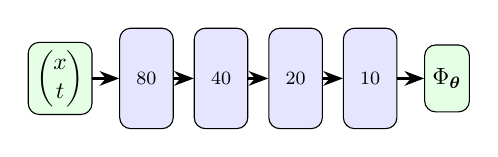
\begin{tikzpicture}[
          node distance=0.8cm, scale=0.85, transform shape,
          layer/.style={draw, rounded corners, minimum width=0.8cm,
                        minimum height=1.5cm, fill=blue!10},
          io/.style={draw, rounded corners, minimum width=0.6cm,
                     minimum height=1.0cm, fill=green!10},
          arr/.style={-{Stealth[length=2.5mm]}, thick}
        ]
          \node[io] (input) {$\begin{pmatrix}x\\t\end{pmatrix}$};
          \node[layer, right=0.4cm of input] (h1) {\footnotesize 80};
          \node[layer, right=0.3cm of h1]    (h2) {\footnotesize 40};
          \node[layer, right=0.3cm of h2]    (h3) {\footnotesize 20};
          \node[layer, right=0.3cm of h3]    (h4) {\footnotesize 10};
          \node[io, right=0.4cm of h4] (output) {$\Phi_{\boldsymbol{\theta}}$};
          \draw[arr] (input) -- (h1);
          \draw[arr] (h1) -- (h2);
          \draw[arr] (h2) -- (h3);
          \draw[arr] (h3) -- (h4);
          \draw[arr] (h4) -- (output);
        \end{tikzpicture}

        \smallskip
        {\scriptsize Output transform: $A\,\tanh(\text{raw})$}
      \end{center}
    \end{column}
  \end{columns}
\end{frame}

% --- Slide 1.3: Where We Were ---
\begin{frame}{Where We Were (Last Meeting --- 25 Feb)}
  \begin{columns}[T]
    \begin{column}{0.48\textwidth}
      \centering
      {\small\textbf{Baseline (Uniform Sampling)}}\\[2pt]
      
\includegraphics[width=\textwidth]{../../project32_qnm_pinn/outputs/pinn/zerilli_l2_paper/error_heatmap.png}
    \end{column}
    \begin{column}{0.48\textwidth}
      \centering
      {\small\textbf{RAD $k\!=\!2$ (Best at Last Meeting)}}\\[2pt]
      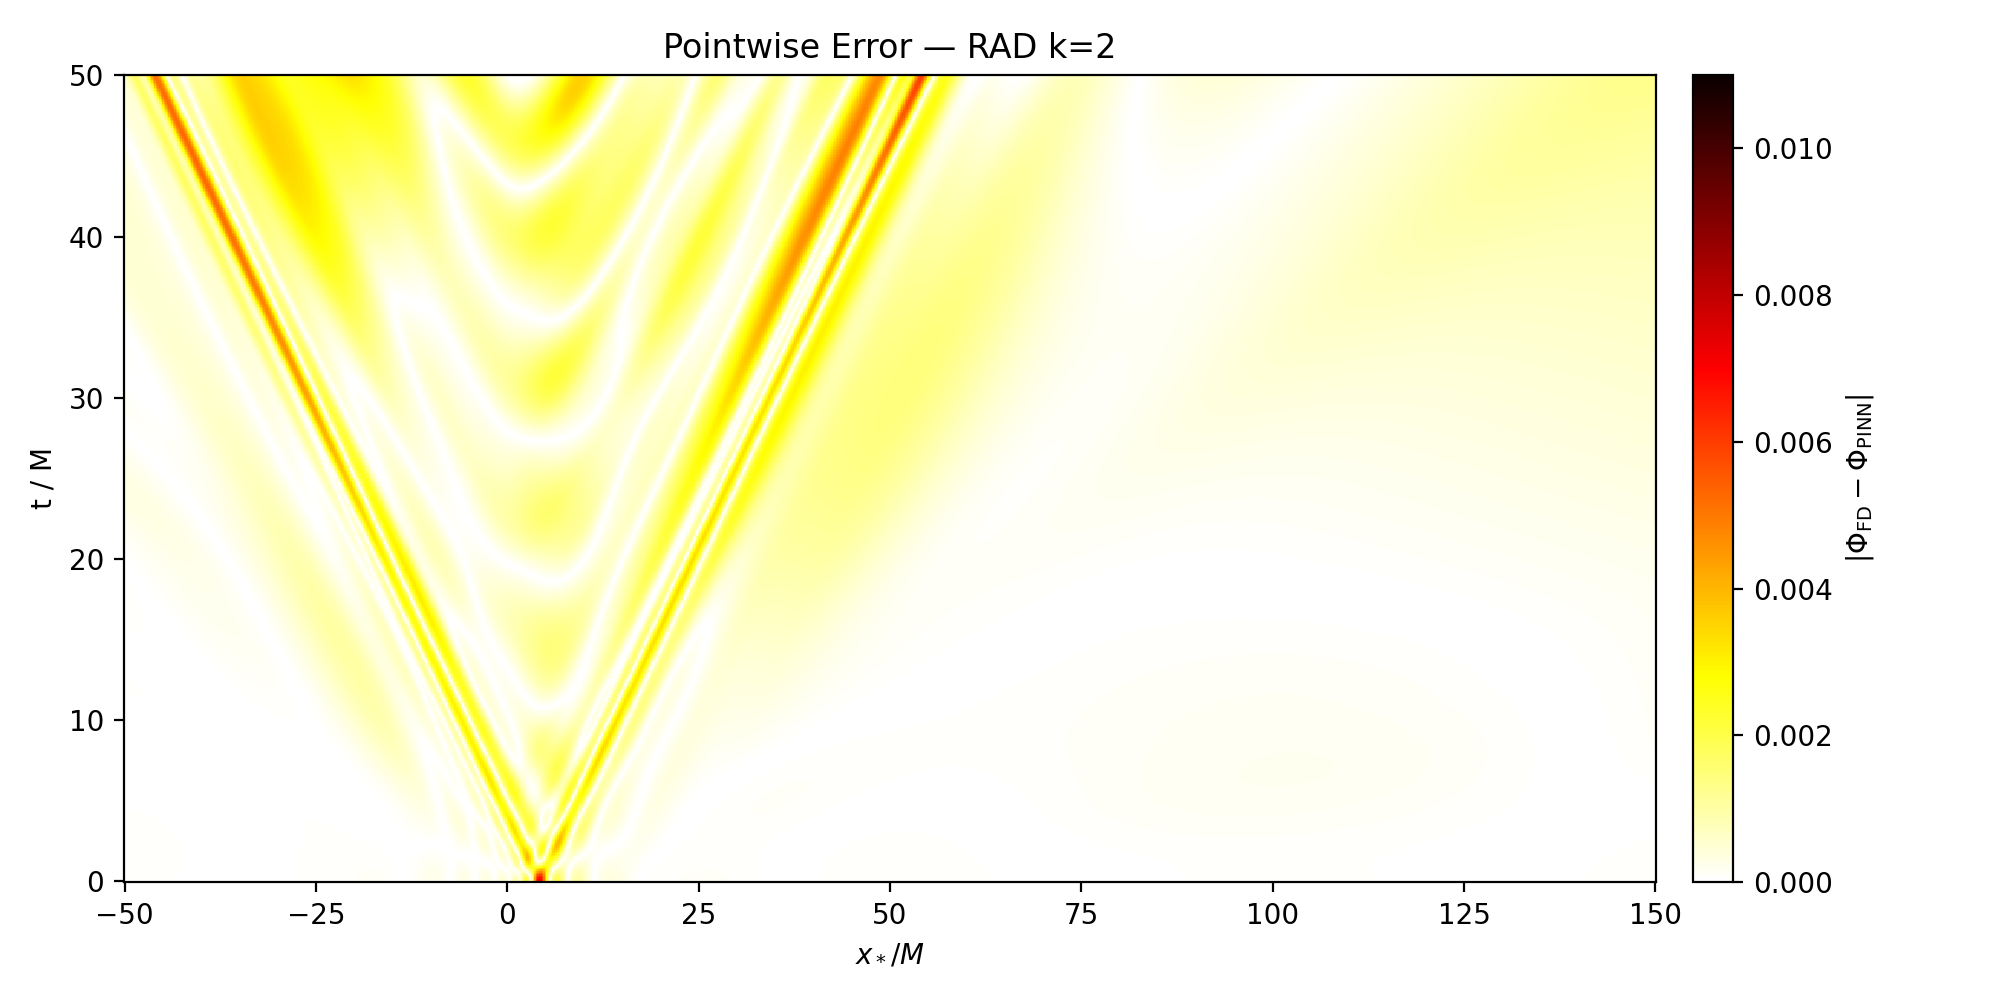
\includegraphics[width=\textwidth]{../outputs/pinn/zerilli_l2_rad_k2/error_heatmap.png}
    \end{column}
  \end{columns}

  \medskip
  \begin{center}
    \footnotesize
    \begin{tabular}{@{}lccc@{}}
      \toprule
      & \textbf{RMSD} & \textbf{M1 $\tau$ err} & \textbf{M2 $\tau$ err} \\
      \midrule
      Uniform baseline & 0.00183 & 5.07\% & 1.50\% \\
      RAD $k\!=\!2$    & 0.00095 \textcolor{darkgreen}{($-$48\%)} & 3.65\% & 1.80\% \\
      \bottomrule
    \end{tabular}
  \end{center}

  \smallskip
  RAD improved \textbf{spatial accuracy} but QNM extraction remained similar.\\
  \textbf{Today:} Three new strategies to push further.
\end{frame}


% ══════════════════════════════════════════════════════════════════
%  SECTION 2 — GREEDY ADAPTIVE RESAMPLING
% ══════════════════════════════════════════════════════════════════
\section{Greedy Adaptive Resampling}

% --- Slide 2.1: Algorithm ---
\begin{frame}{Greedy Resampling --- Algorithm}
  Instead of \textbf{probabilistic} sampling (RAD: $p_i \propto |r_i|^k + c$),
  use \textbf{deterministic top-$N$} selection:

  \medskip
  \begin{enumerate}
    \item Every $P$ steps during Adam, generate $N_{\text{cand}} = 100{,}000$
          random candidates.
    \item Evaluate PDE residual $|r_i|$ at each candidate.
    \item \textbf{Sort by $|r_i|$ descending} --- keep the top $f \times N_r$ points.
    \item Fill the remaining $(1\!-\!f) \times N_r$ slots with \textbf{uniform random} points.
    \item Replace all $N_r = 32{,}000$ domain collocation points.
  \end{enumerate}

  \medskip
  \textbf{Key differences from RAD:}
  \begin{itemize}
    \item \textbf{Deterministic} --- no sampling noise; the most extreme residuals
          are always selected.
    \item \textbf{Single hyperparameter $f$} (fraction) ---
          no tuning of $k$ or $c$.
    \item $f = 0$: uniform; \; $f = 1$: fully greedy.
  \end{itemize}
\end{frame}

% --- Slide 2.2: Sweep Results ---
\begin{frame}{Greedy Resampling --- Sweep Results}
  \begin{columns}[T]
    \begin{column}{0.50\textwidth}
      \begin{center}
        \footnotesize
        \begin{tabular}{@{}lcc@{}}
          \toprule
          \textbf{Configuration} & \textbf{RMSD} & \textbf{vs Baseline} \\
          \midrule
          Uniform (baseline) & 0.00183 & --- \\
          RAD $k\!=\!2$      & 0.00095 & $-$48\% \\
          \midrule
          \rowcolor{green!10}
          Greedy $f\!=\!0.3$ & \textbf{0.00085} & \textbf{$-$54\%} \\
          Greedy $f\!=\!0.5$ & 0.00107 & $-$42\% \\
          Greedy $f\!=\!0.8$+$P$500 & 0.00104 & $-$43\% \\
          \bottomrule
        \end{tabular}
      \end{center}

      \medskip
      \begin{itemize}\small
        \item $f\!=\!0.3$ is optimal: 30\% greedy, 70\% uniform.
        \item Too aggressive ($f \ge 0.5$): loses exploration.
        \item \textbf{Surpasses best RAD} with simpler algorithm.
      \end{itemize}
    \end{column}
    \begin{column}{0.48\textwidth}
      \begin{center}
        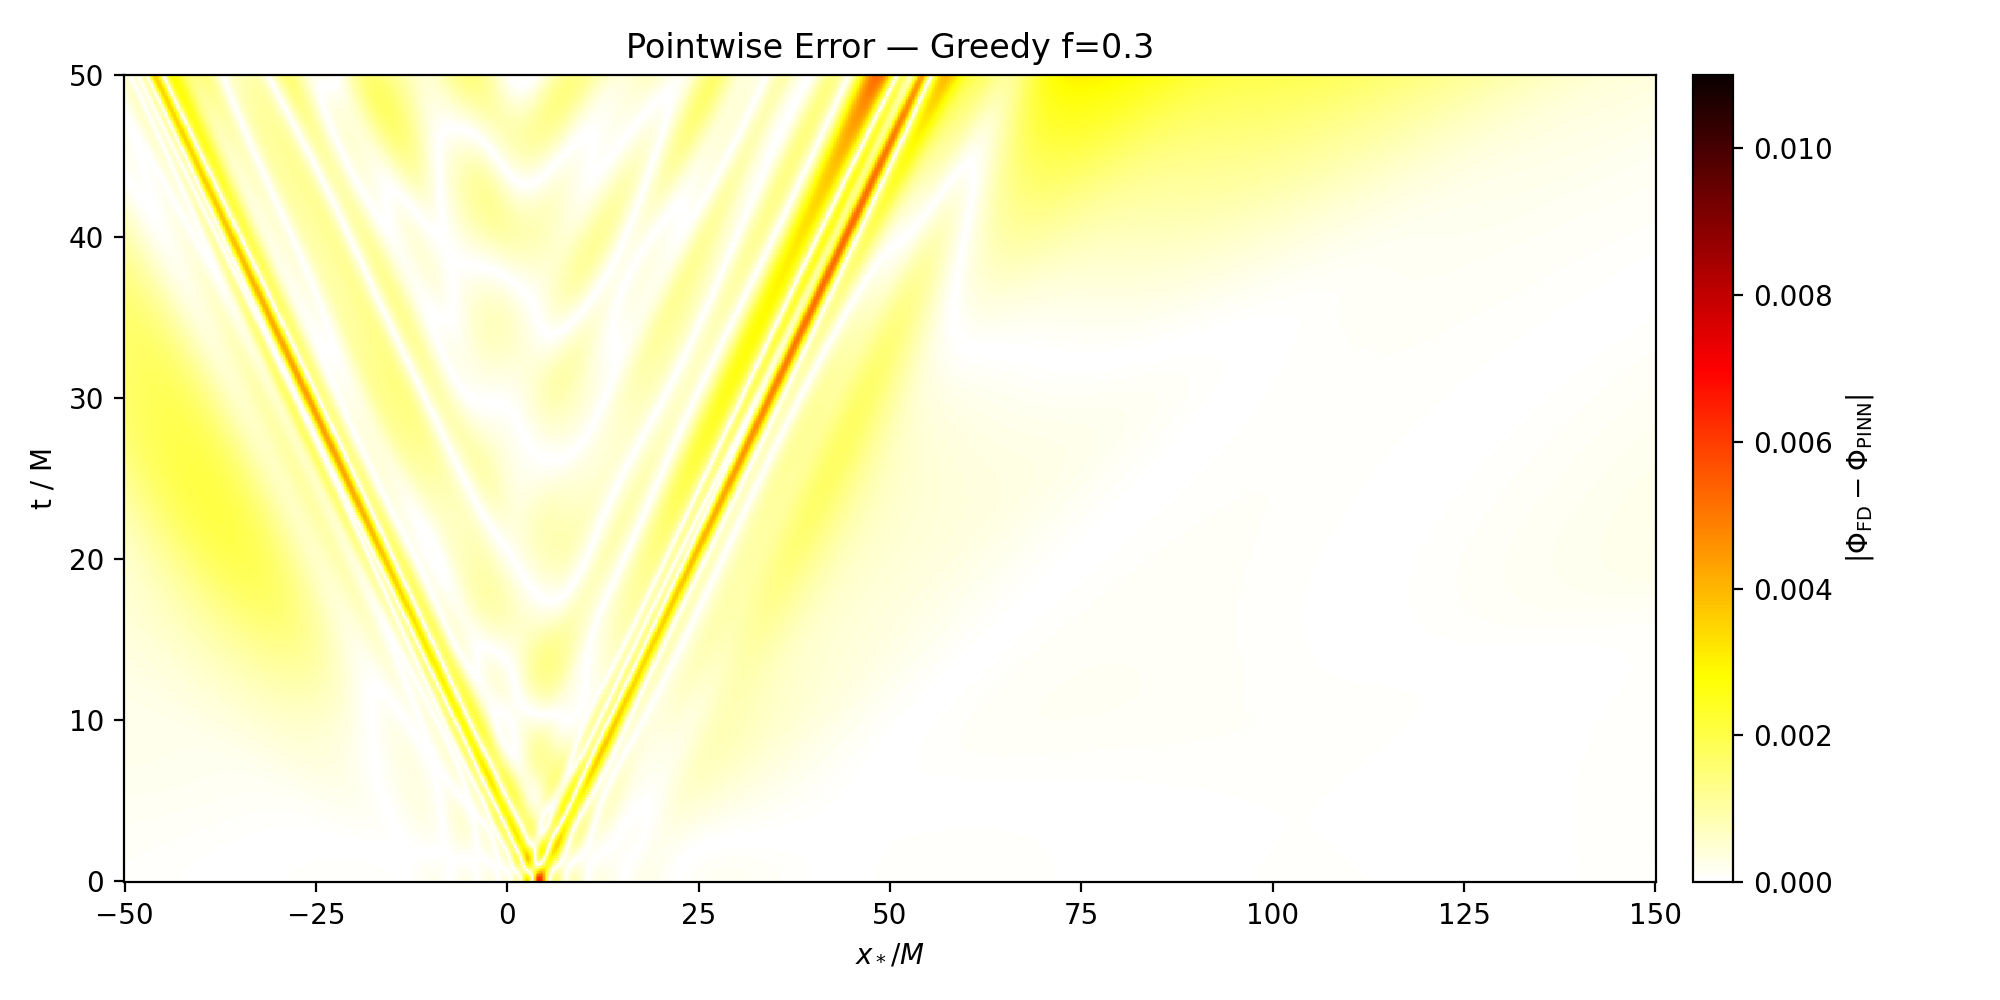
\includegraphics[width=\textwidth]{../outputs/pinn/zerilli_l2_greedy_f03/error_heatmap.png}
        \\{\footnotesize Error heatmap: Greedy $f\!=\!0.3$}
      \end{center}
    \end{column}
  \end{columns}
\end{frame}

% --- Slide 2.3: Extended L-BFGS ---
\begin{frame}{Extended L-BFGS --- Best Forward Model}
  \begin{columns}[T]
    \begin{column}{0.48\textwidth}
      \textbf{Idea:} Double L-BFGS iterations from 15k $\to$ 30k.

      \medskip
      \begin{center}
        \footnotesize
        \begin{tabular}{@{}lcc@{}}
          \toprule
          & \textbf{RMSD} & \textbf{vs Base} \\
          \midrule
          Greedy $f\!=\!0.3$ & 0.00085 & $-$54\% \\
          \rowcolor{green!10}
          \;+ L-BFGS 30k & \textbf{0.00082} & \textbf{$-$55\%} \\
          \bottomrule
        \end{tabular}
      \end{center}

      \medskip
      \begin{itemize}\small
        \item \textbf{Best single-window forward model.}
        \item M1: $\omega$ err\,0.68\%, $\tau$ err\,2.83\%.
        \item M2: $\omega$ err\,1.54\%, $\tau$ err\,1.99\%.
        \item Marginal gain vs.\ $f\!=\!0.3$ alone --- near convergence of the forward approach.
      \end{itemize}
    \end{column}
    \begin{column}{0.50\textwidth}
      \begin{center}
        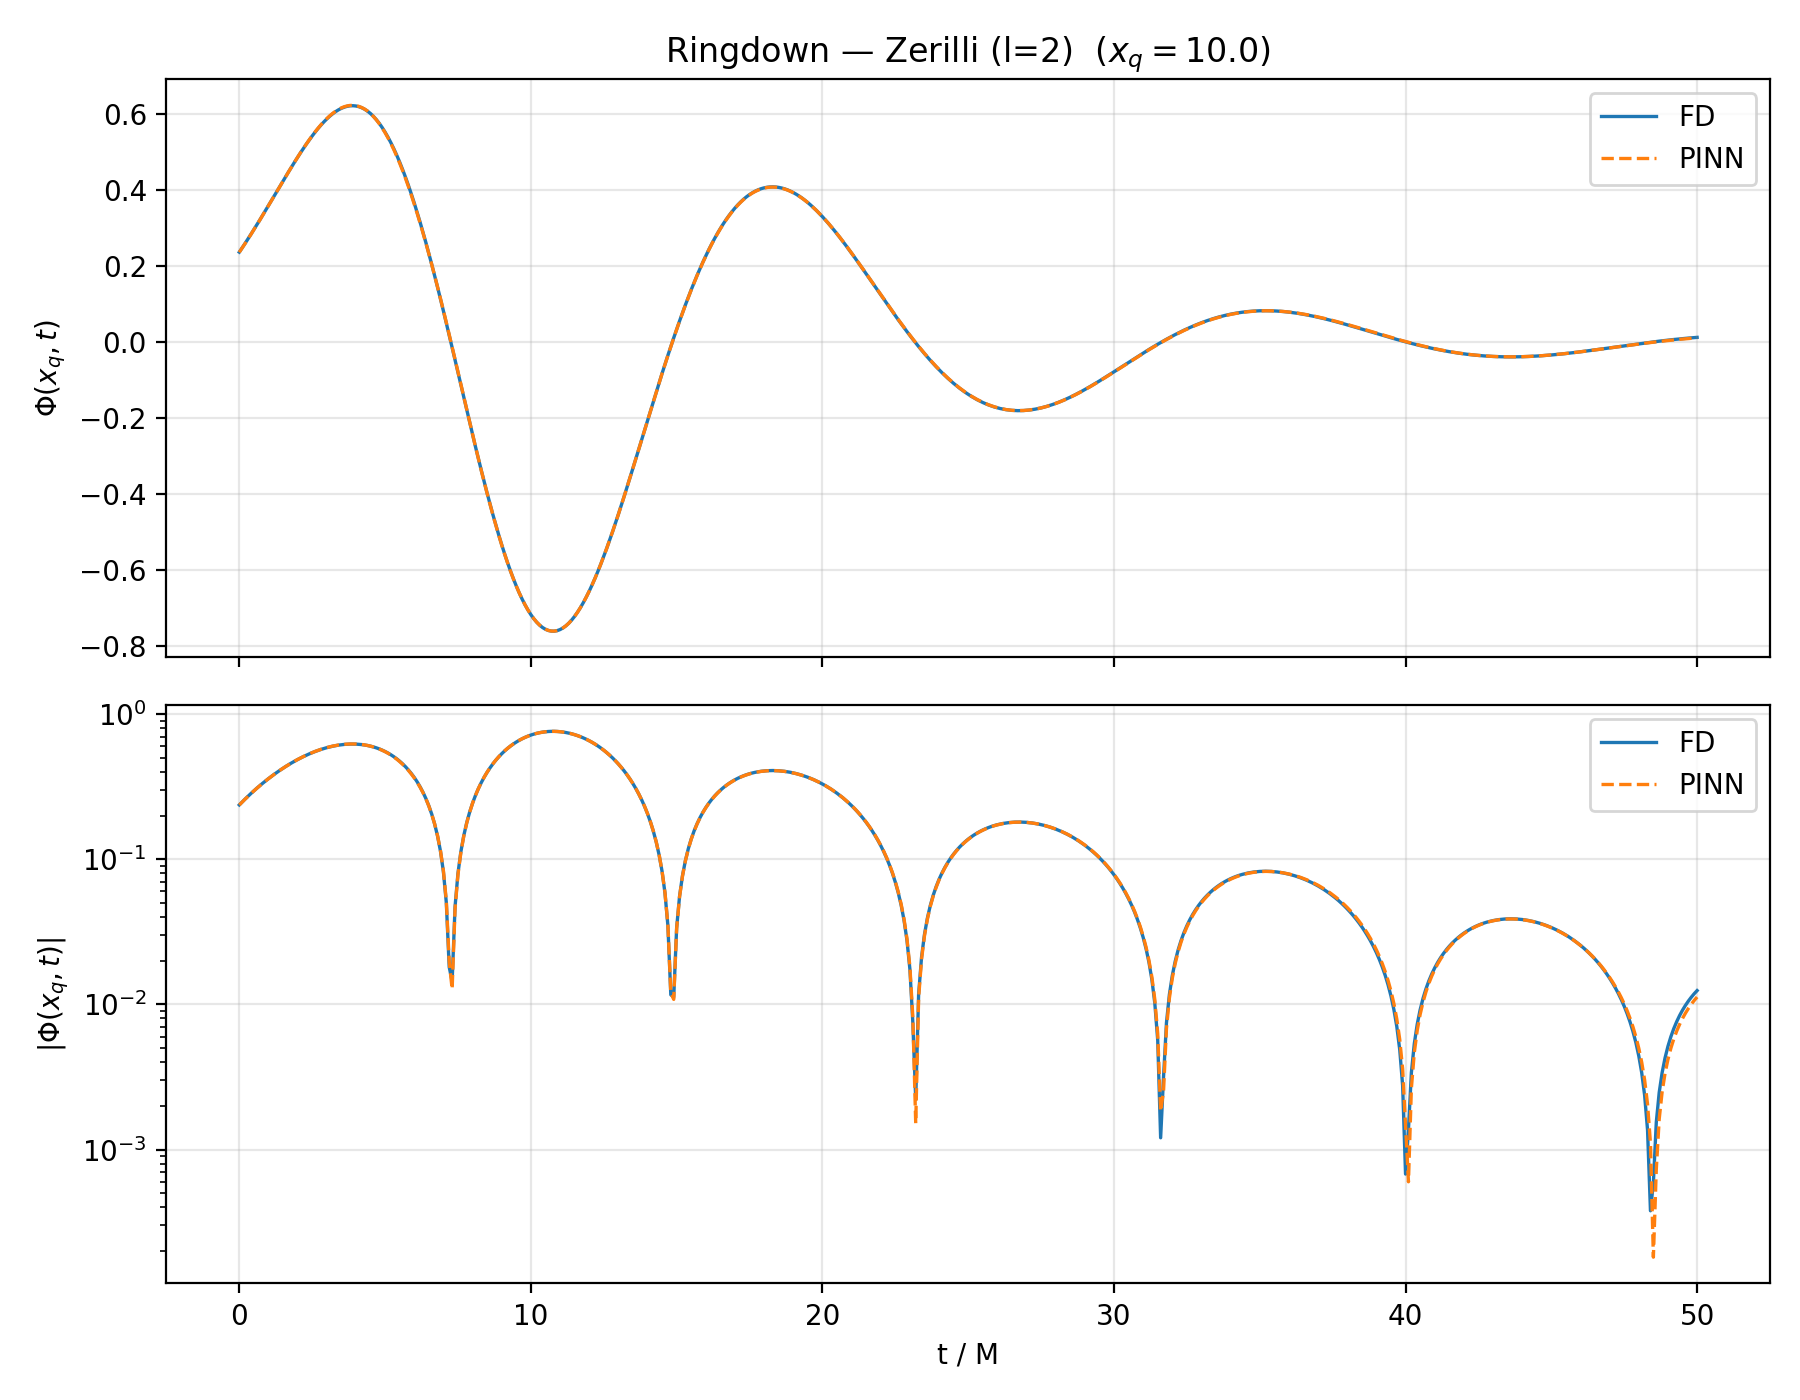
\includegraphics[width=\textwidth]{../outputs/pinn/zerilli_l2_greedy_f03_lbfgs30k/ringdown_overlay.png}
        \\{\footnotesize Ringdown at $x_q = 10M$: Greedy + L-BFGS 30k}
      \end{center}
    \end{column}
  \end{columns}
\end{frame}


% ══════════════════════════════════════════════════════════════════
%  SECTION 3 — CURRICULUM LEARNING
% ══════════════════════════════════════════════════════════════════
\section{Curriculum Learning}

% --- Slide 3.1: Strategy ---
\begin{frame}{Curriculum Learning --- Strategy}
  \textbf{Idea:} Train on sequential time windows instead of the full domain.

  \begin{center}
    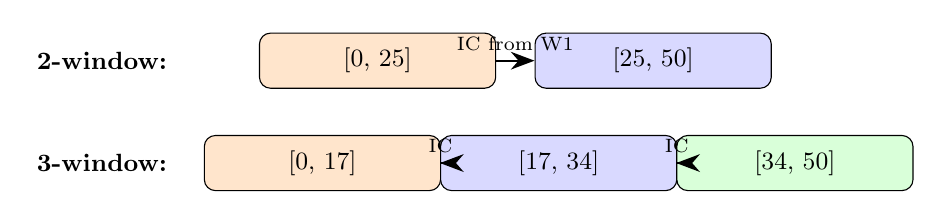
\begin{tikzpicture}[
      box/.style={draw, rounded corners, minimum width=3.0cm,
                  minimum height=0.7cm, font=\small},
      arr/.style={-{Stealth[length=3mm]}, thick}
    ]
      % 2-window
      \node[font=\small\bfseries] at (-2.5, 0) {2-window:};
      \node[box, fill=orange!20] (w1) at (1.0, 0) {$[0,\,25]$};
      \node[box, fill=blue!15]   (w2) at (4.5, 0) {$[25,\,50]$};
      \draw[arr] (w1) -- node[above, font=\scriptsize]{IC from W1} (w2);

      % 3-window
      \node[font=\small\bfseries] at (-2.5, -1.3) {3-window:};
      \node[box, fill=orange!20] (w3a) at (0.3, -1.3) {$[0,\,17]$};
      \node[box, fill=blue!15]   (w3b) at (3.3, -1.3) {$[17,\,34]$};
      \node[box, fill=green!15]  (w3c) at (6.3, -1.3) {$[34,\,50]$};
      \draw[arr] (w3a) -- node[above, font=\scriptsize]{IC} (w3b);
      \draw[arr] (w3b) -- node[above, font=\scriptsize]{IC} (w3c);
    \end{tikzpicture}
  \end{center}

  \medskip
  \begin{itemize}
    \item Each window: independent \pinn{}, full Adam + L-BFGS training.
    \item Previous window's trained output provides \textbf{initial condition}
          for the next.
    \item Uses \textbf{greedy $f\!=\!0.3$} resampling within each window.
    \item Final solution: stitch all windows together.
    \item \textbf{Motivation:} Smaller time domains $\Rightarrow$ easier optimisation
          landscape.
  \end{itemize}
\end{frame}

% --- Slide 3.2: Results ---
\begin{frame}{Curriculum Learning --- Results}
  \begin{center}
    \footnotesize
    \begin{tabular}{@{}lcccccc@{}}
      \toprule
      \textbf{Model} & \textbf{RMSD} & \textbf{vs Base}
        & \textbf{M1 $\omega$ err} & \textbf{M1 $\tau$ err}
        & \textbf{M2 $\omega$ err} & \textbf{M2 $\tau$ err} \\
      \midrule
      Uniform baseline       & 0.00183 & ---     & 1.08\% & 5.07\% & 1.25\% & 1.50\% \\
      Greedy $f\!=\!0.3$     & 0.00085 & $-$54\% & 0.68\% & 2.86\% & 1.54\% & 1.99\% \\
      \midrule
      \rowcolor{green!10}
      Curriculum 2w          & 0.00085 & $-$54\% & 0.70\% & 2.95\% & 1.53\% & 2.11\% \\
      Curriculum 3w          & 0.00098 & $-$47\% & 0.69\% & 3.83\% & 1.59\% & 1.93\% \\
      \bottomrule
    \end{tabular}
  \end{center}

  \medskip
  \begin{itemize}
    \item \textbf{2-window:} Competitive with single-window greedy
          (RMSD $\approx$ 0.00085).
    \item \textbf{3-window:} Slightly worse ---
          error accumulates at window boundaries.
    \item Curriculum works but does \textbf{not outperform}
          the simpler greedy approach.
    \item IC transfer introduces interpolation error at each stitching boundary.
  \end{itemize}
\end{frame}

% --- Slide 3.3: Visuals ---
\begin{frame}{Curriculum Learning --- Ringdown Comparison}
  \begin{columns}[T]
    \begin{column}{0.48\textwidth}
      \begin{center}
        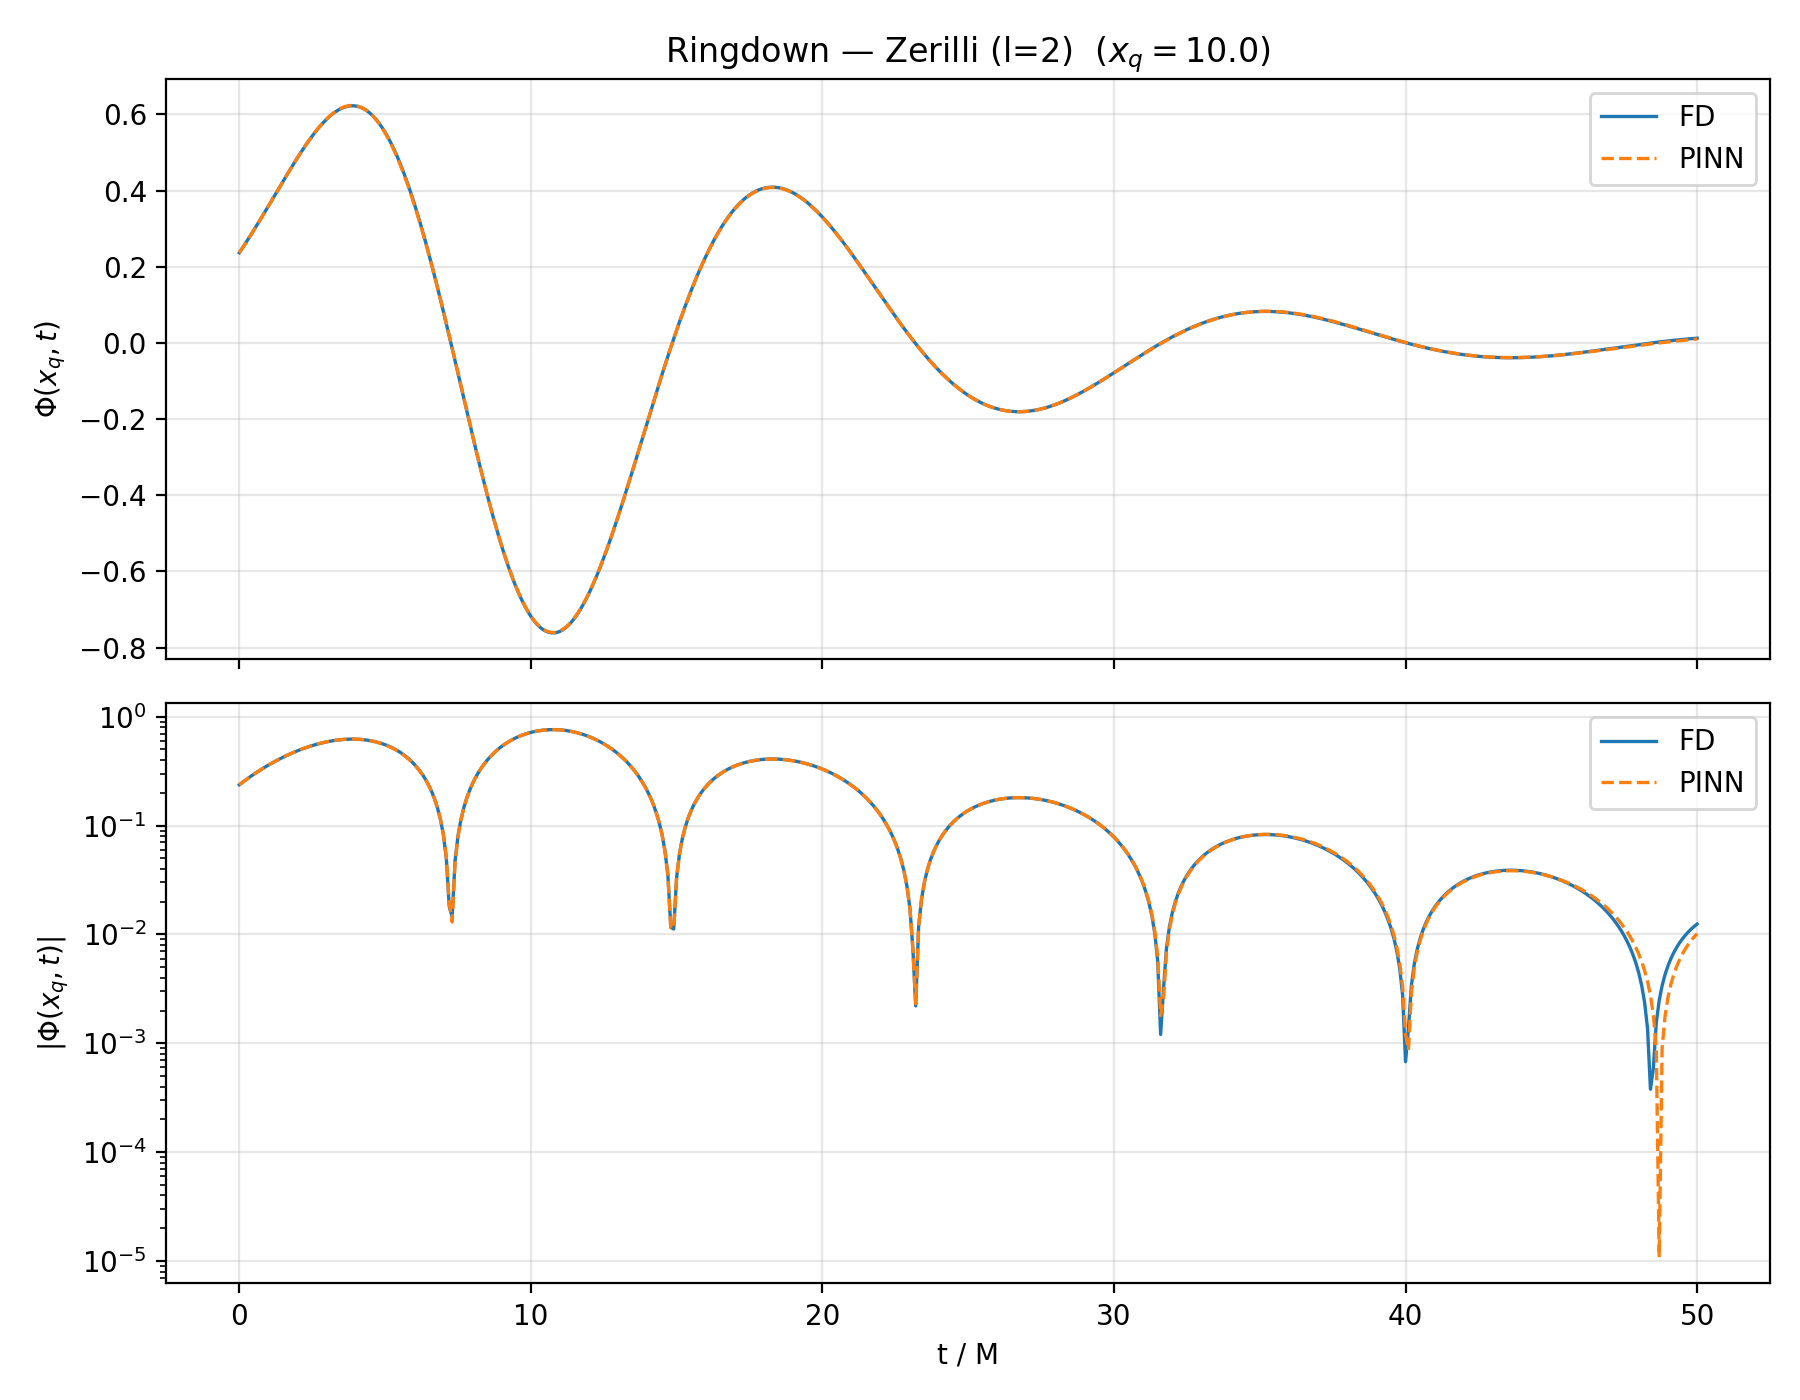
\includegraphics[width=\textwidth]{../outputs/pinn/zerilli_l2_curriculum/ringdown_overlay.png}
        \\{\footnotesize 2-window: $[0,\,25] + [25,\,50]$}
      \end{center}
    \end{column}
    \begin{column}{0.48\textwidth}
      \begin{center}
        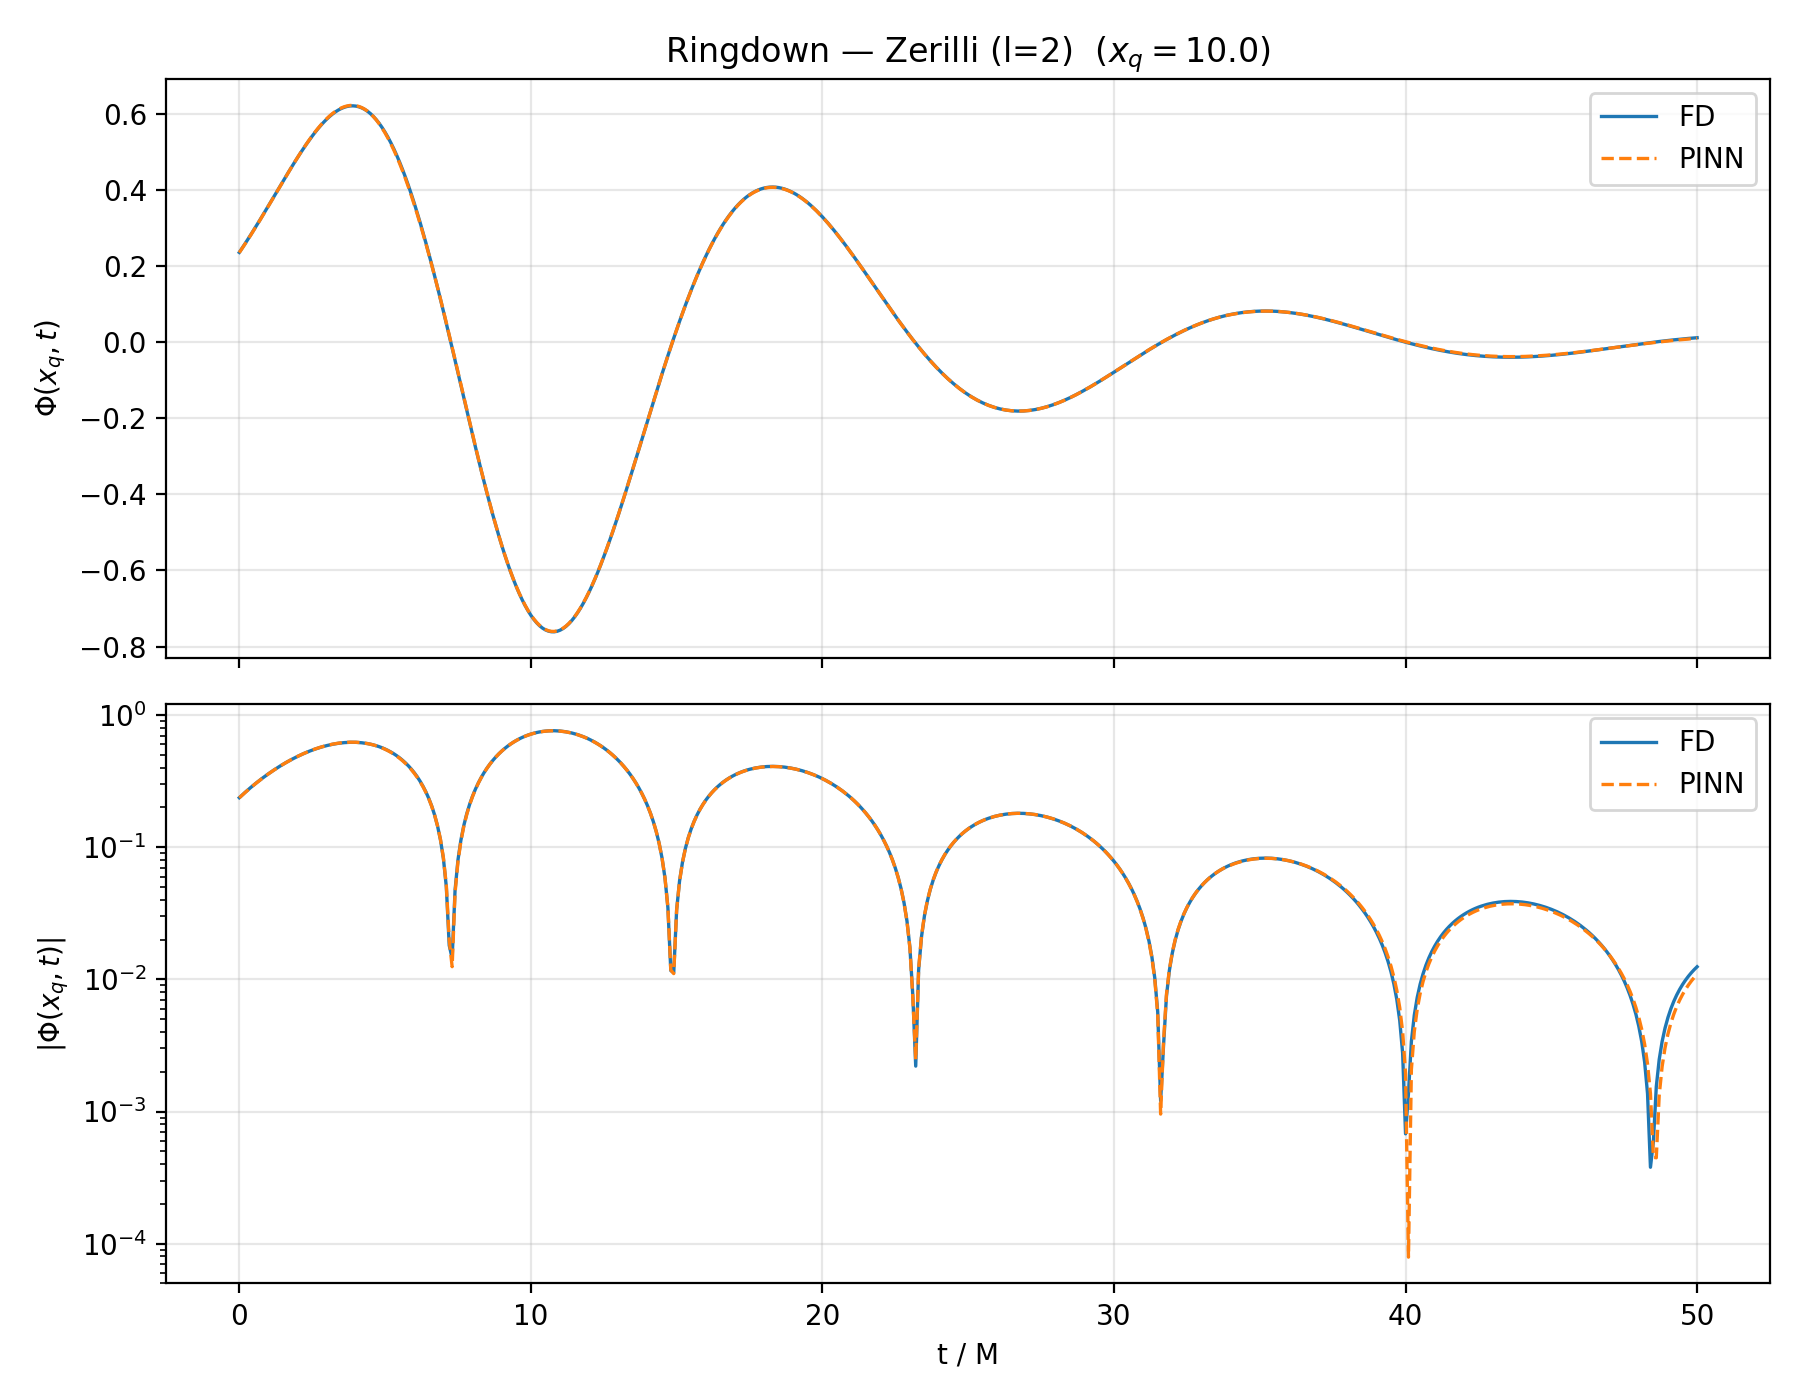
\includegraphics[width=\textwidth]{../outputs/pinn/zerilli_l2_curriculum_3w/ringdown_overlay.png}
        \\{\footnotesize 3-window: $[0,\,17] + [17,\,34] + [34,\,50]$}
      \end{center}
    \end{column}
  \end{columns}

  \medskip
  \begin{center}
    Both match the \fd{} waveform well at $x_q = 10M$.\\
    Small late-time deviations visible in 3-window (right) ---
    error accumulation across boundaries.
  \end{center}
\end{frame}


% ══════════════════════════════════════════════════════════════════
%  SECTION 4 — INVERSE PROBLEM
% ══════════════════════════════════════════════════════════════════
\section{Inverse Problem: Learning Physics from Data}

% --- Slide 4.1: Concept ---
\begin{frame}{A Different Approach --- Inverse PINNs}
  \textbf{Forward \pinn{}:}\; Given PDE parameters
  $\;\to\;$ solve for $\Phi$ $\;\to\;$ extract \qnms{}.

  \medskip
  \textbf{Inverse \pinn{}:}\; Treat PDE parameters as \textbf{learnable}
  --- optimise them alongside the network weights using PDE \emph{and data} losses.

  \medskip
  \begin{center}
    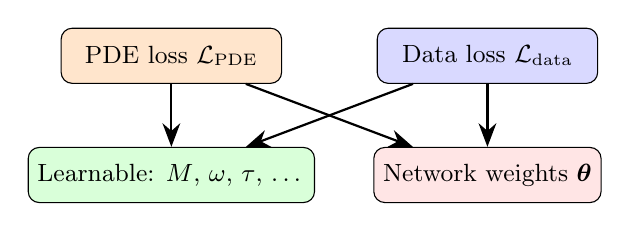
\begin{tikzpicture}[
      box/.style={draw, rounded corners, minimum width=2.8cm,
                  minimum height=0.7cm, font=\small},
      arr/.style={-{Stealth[length=3mm]}, thick}
    ]
      \node[box, fill=orange!20] (pde)    {PDE loss $\mathcal{L}_{\text{PDE}}$};
      \node[box, fill=blue!15, right=1.2cm of pde] (data) {Data loss $\mathcal{L}_{\text{data}}$};
      \node[box, fill=green!15, below=0.8cm of pde]  (params) {Learnable: $M$, $\omega$, $\tau$, \ldots};
      \node[box, fill=red!10,   below=0.8cm of data]  (weights) {Network weights $\boldsymbol{\theta}$};
      \draw[arr] (pde)  -- (params);
      \draw[arr] (data) -- (params);
      \draw[arr] (pde)  -- (weights);
      \draw[arr] (data) -- (weights);
    \end{tikzpicture}
  \end{center}

  \medskip
  \textbf{Total loss} (Inverse PINN --- learn $M$):
  \[
    \mathcal{L} = \underbrace{\lambda_r\mathcal{L}_r + \lambda_{r_x}\mathcal{L}_{r_x}
    + \lambda_{r_t}\mathcal{L}_{r_t}}_{\text{PDE residual (same as forward)}}
    + \underbrace{\lambda_{ic}\mathcal{L}_{ic} + \lambda_{iv}\mathcal{L}_{iv}}_{\text{ICs}}
    + \underbrace{\lambda_{bl}\mathcal{L}_{bl} + \lambda_{br}\mathcal{L}_{br}}_{\text{BCs}}
    + \underbrace{\lambda_{\text{data}}\mathcal{L}_{\text{data}}}_{\text{new}}
  \]
  \begin{itemize}
    \item $\mathcal{L}_{\text{data}} = \text{MSE}\!\bigl(\Phi_{\text{PINN}},\;\Phi_{\text{FD}}\bigr)$
          at 500 random $(x,t)$ points.\quad $\lambda_{\text{data}} = 10$.
    \item PDE loss now depends on $M$ through $V(r)$ and $x(r)$
          $\;\Rightarrow\;$ gradients flow to $M$.
  \end{itemize}
\end{frame}

% --- Slide 4.2: Inverse PINN — Learn M ---
\begin{frame}{Inverse PINN --- Learning Black Hole Mass $M$}
  \begin{columns}[T]
    \begin{column}{0.50\textwidth}
      $M$ enters through the \zer{} potential $V(r)$ and
      the tortoise coordinate $x(r)$.

      \medskip
      \textbf{Setup:}
      \begin{itemize}
        \item Initialise $M = 0.80$ (true: $M = 1.0$).
        \item $M$ is a trainable variable --- optimised
              jointly with~$\boldsymbol{\theta}$.
        \item Same training pipeline + data loss.
      \end{itemize}

      \medskip
      \textbf{Result:}
      \begin{center}
        \begin{tabular}{@{}lc@{}}
          \toprule
          & \textbf{Value} \\
          \midrule
          True $M$    & 1.0000 \\
          Learned $M$ & \textcolor{darkgreen}{0.9986} \\
          Error       & \textcolor{darkgreen}{0.14\%} \\
          \bottomrule
        \end{tabular}
      \end{center}

      \smallskip
      {\small RMSD\,=\,0.00408 (higher than forward ---
      different objective).}
    \end{column}
    \begin{column}{0.48\textwidth}
      \begin{center}
        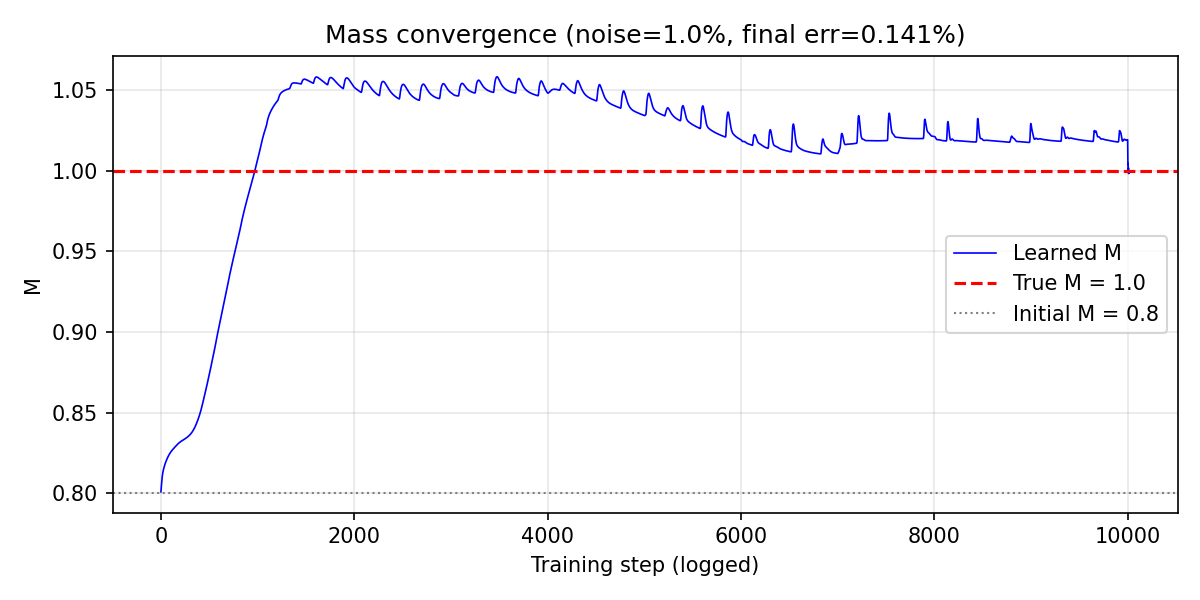
\includegraphics[width=\textwidth]{../outputs/pinn/zerilli_l2_inverse/M_convergence.png}
        \\{\footnotesize $M$ converges from 0.80 to 0.9986}
      \end{center}
    \end{column}
  \end{columns}
\end{frame}

% --- Slide 4.3: Inverse PINN + Ringdown Template — Concept ---
\begin{frame}{Inverse PINN + Ringdown Template --- Concept}
  \textbf{Learn simultaneously:} $M$ (via PDE) and $\omega$, $\tau$, $A$, $\phi_0$
  (via ringdown template).

  \medskip
  \textbf{Total loss:}
  \[
    \mathcal{L} = \underbrace{\lambda_r\mathcal{L}_r + \lambda_{r_x}\mathcal{L}_{r_x}
    + \lambda_{r_t}\mathcal{L}_{r_t}}_{\text{PDE residual (depends on $M$)}}
    + \underbrace{\lambda_{ic}\mathcal{L}_{ic} + \lambda_{iv}\mathcal{L}_{iv}}_{\text{ICs}}
    + \underbrace{\lambda_{bl}\mathcal{L}_{bl} + \lambda_{br}\mathcal{L}_{br}}_{\text{BCs}}
    + \underbrace{\lambda_{\text{data}}\mathcal{L}_{\text{data}}}_{\substack{\text{match fixed}\\\text{FD data}}}
    + \underbrace{\lambda_{\text{ring}}\mathcal{L}_{\text{ring}}}_{\substack{\text{match learnable}\\\text{ringdown ansatz}}}
  \]

  \begin{itemize}
    \item $\mathcal{L}_{\text{data}} = \text{MSE}\!\bigl(\Phi_{\text{PINN}},\;\Phi_{\text{FD}}^{\text{noisy}}\bigr)$
          --- compares against \textbf{fixed} noisy FD observations
          at 500 random $(x,t)$ points across the full domain.\quad $\lambda_{\text{data}} = 10$.
    \item $\mathcal{L}_{\text{ring}} = \text{MSE}\!\bigl(\Phi_{\text{PINN}}(x_0, t),\;
          A\,e^{-t/\tau}\cos(\omega\,t + \phi_0)\bigr)$
          --- compares against a \textbf{learnable} damped-sinusoid template
          at one point $x_0\!=\!10$, late times $t \in [10, 50]$ only (200 pts).\quad $\lambda_{\text{ring}} = 1$.
    \item $M$ learned through $V(x; M)$ in PDE; \;$\omega$, $\tau$, $A$, $\phi_0$ learned through $\mathcal{L}_{\text{ring}}$.
  \end{itemize}
\end{frame}

% --- Slide 4.4a: Inverse PINN + Ringdown Template — Results ---
\begin{frame}{Inverse PINN + Ringdown Template --- Results}
  \begin{columns}[T]
    \begin{column}{0.38\textwidth}
      \textbf{Parameter recovery:}
      \begin{center}
        \small
        \begin{tabular}{@{}lccc@{}}
          \toprule
          & \textbf{Init} & \textbf{Learned} & \textbf{Err} \\
          \midrule
          $M$        & 0.80 & 1.004  & 0.41\% \\
          $\omega M$ & 0.30 & 0.382  & 2.23\% \\
          $\tau/M$   & 8.0  & 11.89  & 5.77\% \\
          \bottomrule
        \end{tabular}
      \end{center}

      \medskip
      \textbf{Key result:}\\
      Prony extraction from the waveform gives
      $\tau$ error = \textcolor{darkgreen}{\textbf{1.52\%}}
      --- \textbf{best of all experiments!}
    \end{column}
    \begin{column}{0.60\textwidth}
      \begin{center}
        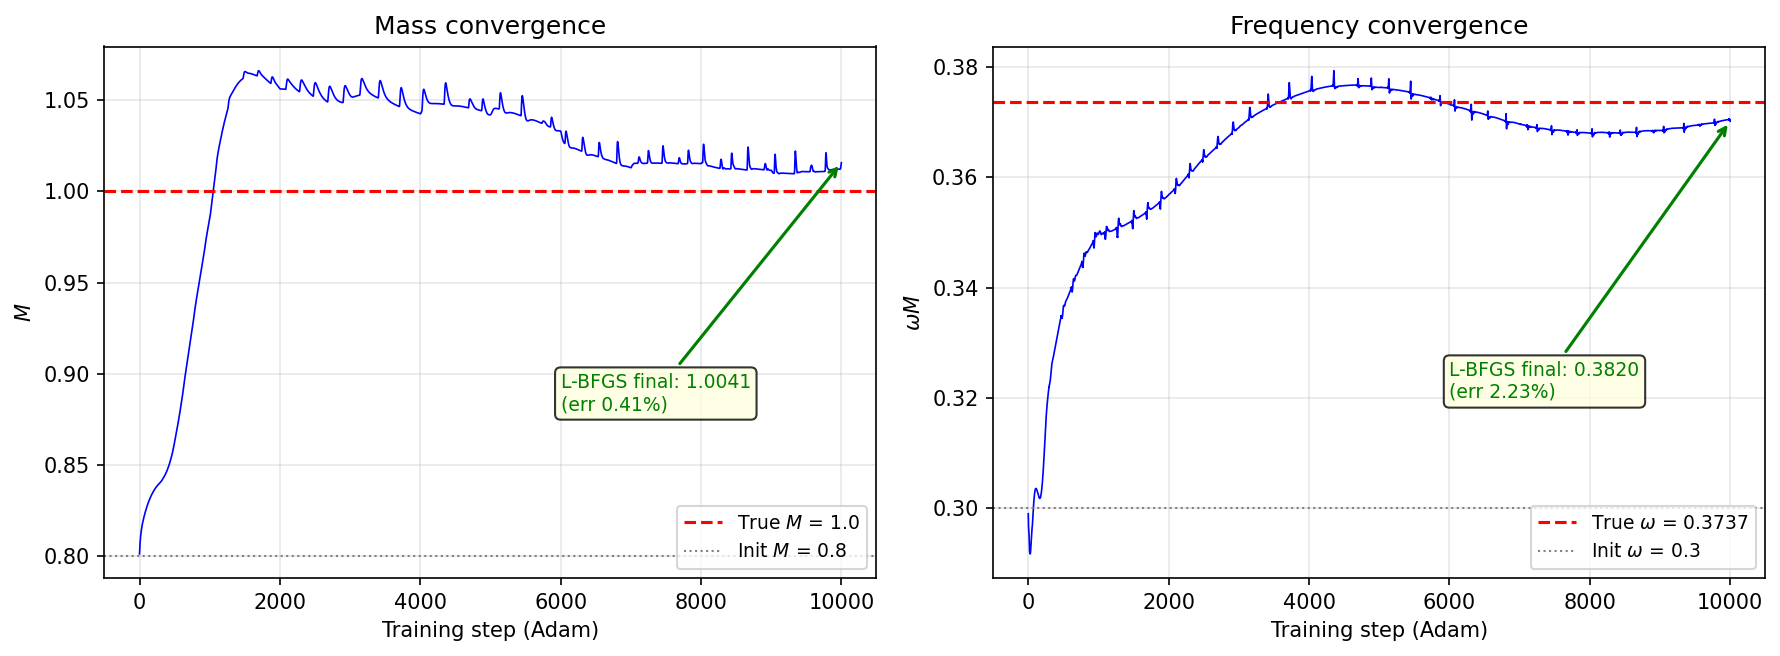
\includegraphics[width=\textwidth]{../outputs/pinn/zerilli_l2_inverse_qnm/param_M_omega.png}
        \\{\footnotesize $M$ and $\omega$ convergence from initial guesses.
        Green line marks Adam\,$\to$\,L-BFGS transition.}
      \end{center}
    \end{column}
  \end{columns}
\end{frame}

% --- Slide 4.4b: Damping time convergence ---
\begin{frame}{Inverse PINN + Ringdown Template --- Damping Time}
  \begin{center}
    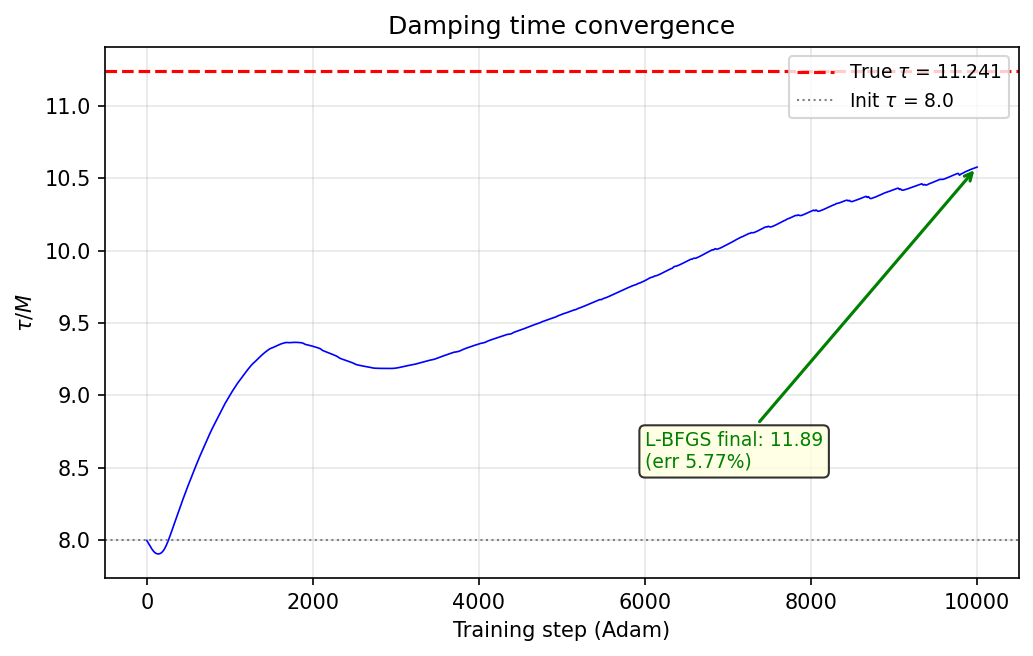
\includegraphics[width=0.65\textwidth]{../outputs/pinn/zerilli_l2_inverse_qnm/param_tau.png}
    \\[4pt]
    {\footnotesize $\tau$ convergence from initial guess $\tau_0=8.0$ to learned $\tau=11.89$
    (true: $11.24$, error $5.77\%$).
    Green line marks Adam\,$\to$\,L-BFGS transition.}
  \end{center}

  \medskip
  \begin{itemize}
    \item Adam brings $\tau$ from 8.0 to $\sim$10.6 (10\,000 steps).
    \item L-BFGS refines to 11.89 (15k iters, converges rapidly with second-order curvature).
    \item Despite 5.77\% learned parameter error, Prony extraction from the
          \emph{regularised} waveform gives $\tau$ error =
          \textcolor{darkgreen}{\textbf{1.52\%}}.
  \end{itemize}
\end{frame}

% --- Slide 4.4: Why Template Helps Prony ---
\begin{frame}{Why Does the Template Loss Help Prony?}
  \begin{columns}[T]
    \begin{column}{0.48\textwidth}
      \textbf{The problem with forward models:}
      \begin{itemize}
        \item At late times, signal decays to $\sim\!10^{-3}$--$10^{-4}$.
        \item PDE residual noise is $O(10^{-3})$ ---
              comparable to the signal itself.
        \item Prony fits $\ln|\text{peaks}|$ vs.\ $t$
              $\;\Rightarrow\;$ noise corrupts the slope.
        \item \textbf{Result:} $\tau$ systematically underestimated
              by $\sim$3--5\%.
      \end{itemize}
    \end{column}
    \begin{column}{0.48\textwidth}
      \textbf{What the template loss does:}
      \begin{itemize}
        \item Forces $\Phi \approx A\,e^{-t/\tau}\cos(\omega t + \phi_0)$
              at late times.
        \item \textbf{Regularises} the exponential decay envelope.
        \item Prony reads a clean decay $\;\Rightarrow\;$ accurate $\tau$.
      \end{itemize}
    \end{column}
  \end{columns}
\end{frame}

% --- Slide 4.5: Why Worst on Method 2 ---
\begin{frame}{Template Loss --- Trade-off Between Extraction Methods}
  \textbf{But why is Inverse PINN + Ringdown Template the \emph{worst} on Method 2?}

  \begin{itemize}
    \item The template loss overwrites PDE-derived physics with the
          \textbf{learned} (imperfect) parameters $\omega$, $\tau$, $A$, $\phi_0$.
    \item Method 2 (curve fit) reads those parameters \emph{back} from the
          waveform --- it recovers the learned values, not the true values.
    \item M2 $\tau$ error = 5.27\% (worst of all experiments).
  \end{itemize}

  \bigskip
  \begin{center}
    \fbox{\parbox{0.75\textwidth}{\centering
      \textbf{Prony} $\;\leftrightarrow\;$ waveform cleanliness
      (late-time envelope shape)\\[4pt]
      \textbf{Method 2} $\;\leftrightarrow\;$ PDE-encoded physics
      (overall waveform fidelity)
    }}
  \end{center}

  \medskip
  \begin{center}
    \textbf{No single method dominates both extraction approaches.}
  \end{center}
\end{frame}


% ══════════════════════════════════════════════════════════════════
%  SECTION 5 — COMPREHENSIVE RANKINGS
% ══════════════════════════════════════════════════════════════════
\section{Comprehensive Results}

% --- Slide 5.1: RMSD Rankings ---
\begin{frame}{RMSD Rankings --- All Forward Models}
  \begin{center}
    \footnotesize
    \begin{tabular}{@{}rlcc@{}}
      \toprule
      \textbf{Rank} & \textbf{Experiment} & \textbf{RMSD} & \textbf{vs Baseline} \\
      \midrule
      \rowcolor{green!10}
      1  & Greedy $f\!=\!0.3$ + L-BFGS 30k & \textbf{0.000817} & $-$55\% \\
      2  & Curriculum 2-window              & 0.000845          & $-$54\% \\
      3  & Greedy $f\!=\!0.3$               & 0.000850          & $-$54\% \\
      4  & RAD $k\!=\!2$                    & 0.000948          & $-$48\% \\
      5  & Curriculum 3-window              & 0.000976          & $-$47\% \\
      6  & Greedy $f\!=\!0.8$ + $P$500      & 0.001041          & $-$43\% \\
      7  & RAD $k\!=\!2$ + $P$500           & 0.001052          & $-$43\% \\
      8  & Greedy $f\!=\!0.5$               & 0.001066          & $-$42\% \\
      9  & RAD default                      & 0.001150          & $-$37\% \\
      10 & RAD anchor                       & 0.001412          & $-$23\% \\
      11 & Greedy $f\!=\!0.8$               & 0.001647          & $-$10\% \\
      \rowcolor{red!5}
      12 & \textbf{Paper baseline}          & 0.001831          & ---     \\
      \bottomrule
    \end{tabular}
  \end{center}

  \medskip
  \begin{itemize}\small
    \item All adaptive methods improve over uniform sampling.
    \item \textbf{Greedy $f\!=\!0.3$ + L-BFGS 30k}: best spatial accuracy.
    \item Inverse models (RMSD $\sim$0.004--0.005) not shown --- different objective.
  \end{itemize}
\end{frame}

% --- Slide 5.2: Method 1 (Prony) Rankings ---
\begin{frame}{Method 1 (Prony) Rankings --- $\omega$ and $\tau$ Accuracy}
  \begin{center}
    \scriptsize
    \begin{tabular}{@{}rlccc@{}}
      \toprule
      & \textbf{Experiment}
        & $\boldsymbol{\omega}$ \textbf{err\,\%}
        & $\boldsymbol{\tau}$ \textbf{err\,\%}
        & \textbf{Avg} \\
      \midrule
      \rowcolor{green!10}
      1  & Inverse PINN + Ringdown Template      & 1.02         & \textbf{1.52} & \textbf{1.27} \\
      2  & RAD anchor                       & \textbf{0.61} & 2.82          & 1.72 \\
      3  & Greedy $f\!=\!0.3$ + L-BFGS 30k & 0.68          & 2.83          & 1.76 \\
      4  & Greedy $f\!=\!0.3$               & 0.68          & 2.86          & 1.77 \\
      5  & Greedy $f\!=\!0.8$ + $P$500      & 0.69          & 2.85          & 1.77 \\
      6  & RAD $k\!=\!2$ + $P$500           & 0.68          & 2.88          & 1.78 \\
      7  & Curriculum 2-window              & 0.70          & 2.95          & 1.82 \\
      8  & Greedy $f\!=\!0.5$               & 0.74          & 3.65          & 2.20 \\
      9  & RAD $k\!=\!2$                    & 0.85          & 3.65          & 2.25 \\
      10 & Curriculum 3-window              & 0.69          & 3.83          & 2.26 \\
      11 & RAD default                      & 0.80          & 3.77          & 2.29 \\
      12 & Greedy $f\!=\!0.8$               & 0.89          & 4.08          & 2.49 \\
      \rowcolor{red!5}
      13 & Paper baseline                   & 1.08          & 5.07          & 3.08 \\
      \bottomrule
    \end{tabular}
  \end{center}

  \smallskip
  \begin{itemize}\small
    \item \textbf{Inverse PINN + Ringdown Template}: best Prony $\tau$ (1.52\%) via template regularisation.
    \item Forward models cluster at 1.7--2.3\% average error.
  \end{itemize}
\end{frame}

% --- Slide 5.3: Method 2 (Curve Fit) Rankings ---
\begin{frame}{Method 2 (Curve Fit) Rankings --- $\omega$ and $\tau$ Accuracy}
  \begin{center}
    \scriptsize
    \begin{tabular}{@{}rlccc@{}}
      \toprule
      & \textbf{Experiment}
        & $\boldsymbol{\omega}$ \textbf{err\,\%}
        & $\boldsymbol{\tau}$ \textbf{err\,\%}
        & \textbf{Avg} \\
      \midrule
      \rowcolor{green!10}
      1  & Paper baseline                    & 1.25          & \textbf{1.50} & \textbf{1.38} \\
      2  & RAD default                       & 1.44          & 1.65          & 1.55 \\
      3  & Greedy $f\!=\!0.8$                & \textbf{1.42} & 1.80          & 1.61 \\
      4  & RAD $k\!=\!2$                     & 1.43          & 1.80          & 1.61 \\
      5  & Greedy $f\!=\!0.5$                & 1.50          & 1.89          & 1.70 \\
      6  & Curriculum 3-window               & 1.59          & 1.93          & 1.76 \\
      7  & Greedy $f\!=\!0.3$                & 1.54          & 1.99          & 1.76 \\
      8  & RAD anchor                        & 1.57          & 1.96          & 1.77 \\
      9  & Greedy $f\!=\!0.3$ + L-BFGS 30k  & 1.54          & 1.99          & 1.77 \\
      10 & Curriculum 2-window               & 1.53          & 2.11          & 1.82 \\
      11 & Greedy $f\!=\!0.8$ + $P$500       & 1.58          & 2.21          & 1.90 \\
      12 & RAD $k\!=\!2$ + $P$500            & 1.57          & 2.24          & 1.90 \\
      13 & Inverse PINN                      & 1.66          & 2.49          & 2.07 \\
      \rowcolor{red!5}
      14 & Inverse PINN + Ringdown Template       & 2.18          & 5.27          & 3.72 \\
      \bottomrule
    \end{tabular}
  \end{center}

  \smallskip
  \begin{itemize}\small
    \item \textbf{Paper baseline leads M2} --- template regularisation \emph{hurts} curve fitting.
    \item Inverse PINN + Ringdown Template: best on M1 but \textbf{worst on M2}
          (template encodes imperfect learned params).
  \end{itemize}
\end{frame}


% ══════════════════════════════════════════════════════════════════
%  SECTION 6 — SUMMARY
% ══════════════════════════════════════════════════════════════════
\section{Summary \& Outlook}

% --- Slide 6.1: Key Takeaways ---
\begin{frame}{Key Takeaways}
  \begin{enumerate}
    \item \textbf{Greedy $f\!=\!0.3$ + Extended L-BFGS:}
          Best spatial accuracy (RMSD $-$55\%).
          Simple, effective, no complex hyperparameter tuning.

    \medskip
    \item \textbf{Curriculum learning:}
          Competitive with greedy (2-window), but does not outperform it.
          Error accumulates with more windows.

    \medskip
    \item \textbf{Inverse PINN with template loss:}
          Best Prony $\tau$ extraction (1.52\% error).
          Template regularisation cleans the late-time waveform.

    \medskip
    \item \textbf{No single method dominates all metrics.}
          \begin{itemize}
            \item Best RMSD $\neq$ best \qnm{} extraction.
            \item Best M1 $\neq$ best M2.
            \item The extraction method matters as much as the solver.
          \end{itemize}
  \end{enumerate}

  \medskip
  \textbf{Future directions:}
  Extend to Kerr \bh{}s?\;
  Multi-mode ($\ell > 2$) extraction?
\end{frame}

% ══════════════════════════════════════════════════════════════════
%  THANK YOU
% ══════════════════════════════════════════════════════════════════
\begin{frame}{}
  \begin{center}
    {\Large Thank you}

    \bigskip
    Questions?
  \end{center}
\end{frame}

% ══════════════════════════════════════════════════════════════════
%  APPENDIX
% ══════════════════════════════════════════════════════════════════
\renewcommand{\mainend}{\inserttotalframenumber}
\makeatletter
\immediate\write\@auxout{\string\gdef\string\mainend{\the\c@framenumber}}
\makeatother

\appendix
\setbeamertemplate{footline}{%
  \hfill%
  \usebeamerfont{footline}%
  Appendix%
  \hspace*{4pt}\vskip4pt%
}

% --- Appendix: QNM Method 1 ---
\begin{frame}{Appendix: QNM Extraction --- Method 1 (FFT + Envelope)}
  \small
  Extract $\omega$ and $\tau$ \textbf{independently} from the late-time waveform
  $\Phi(x_q,t)$.

  \medskip
  \textbf{Step 1 --- Estimate $\omega$ via FFT:}
  \begin{enumerate}
    \item Window the signal; subtract the mean; apply Hann window.
    \item Zero-pad by $64\times$ and compute the real FFT.
    \item Peak frequency refined with \textbf{parabolic interpolation}.
    \item $\omega = 2\pi f_{\text{peak}}$.
  \end{enumerate}

  \medskip
  \textbf{Step 2 --- Estimate $\tau$ via log-linear envelope fit:}
  \begin{enumerate}
    \item Find local maxima of $|\Phi(x_q,t)|$ (envelope peaks).
    \item $\ln|y_{\text{peaks}}| = \ln A - t/\tau$.
    \item Linear fit $\;\Rightarrow\;$ slope $m = -1/\tau$, hence $\tau = -1/m$.
  \end{enumerate}
\end{frame}

% --- Appendix: QNM Method 2 ---
\begin{frame}{Appendix: QNM Extraction --- Method 2 (Nonlinear Curve Fit)}
  \small
  Fit the full damped-cosine model \textbf{simultaneously}:
  \[
    \Phi(x_q,t) \;\approx\; A\,e^{-t/\tau}\,\cos(\omega\,t + \phi).
  \]

  \textbf{Procedure:}
  \begin{enumerate}
    \item Initial guesses from Method~1: $\omega_0$, $\tau_0$,
          $A_0 = \max|\Phi|$, $\phi_0 = 0$.
    \item \texttt{scipy.optimize.curve\_fit} (Levenberg--Marquardt)
          with four free parameters.
  \end{enumerate}

  \medskip
  \textbf{Advantages:} All parameters fitted jointly; uses every data point.\\
  \textbf{Disadvantage:} Requires good initial guesses; non-robust to noise.
\end{frame}

% --- Appendix: Error Heatmaps ---
\begin{frame}{Appendix: Error Heatmap Gallery}
  \begin{columns}[T]
    \begin{column}{0.32\textwidth}
      \centering
      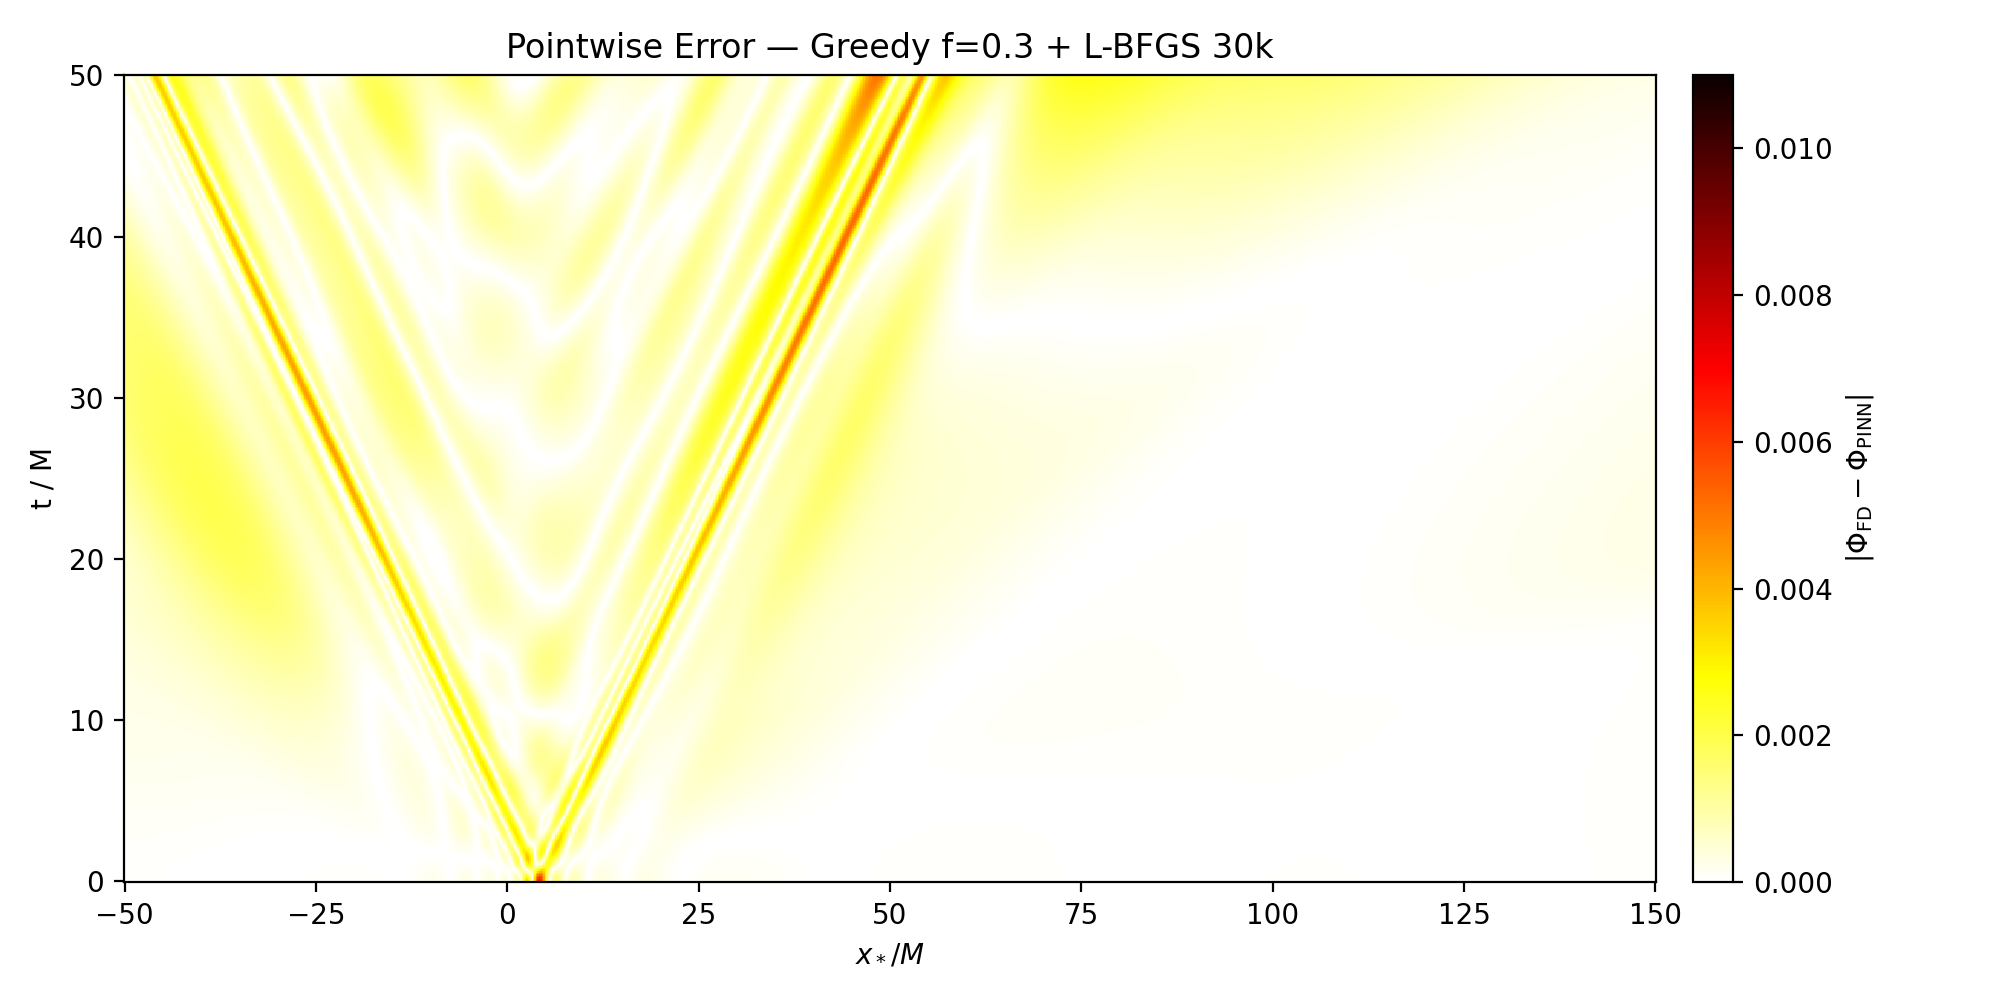
\includegraphics[width=\textwidth]{../outputs/pinn/zerilli_l2_greedy_f03_lbfgs30k/error_heatmap.png}
      \\{\tiny Greedy $f\!=\!0.3$ + L-BFGS 30k}
    \end{column}
    \begin{column}{0.32\textwidth}
      \centering
      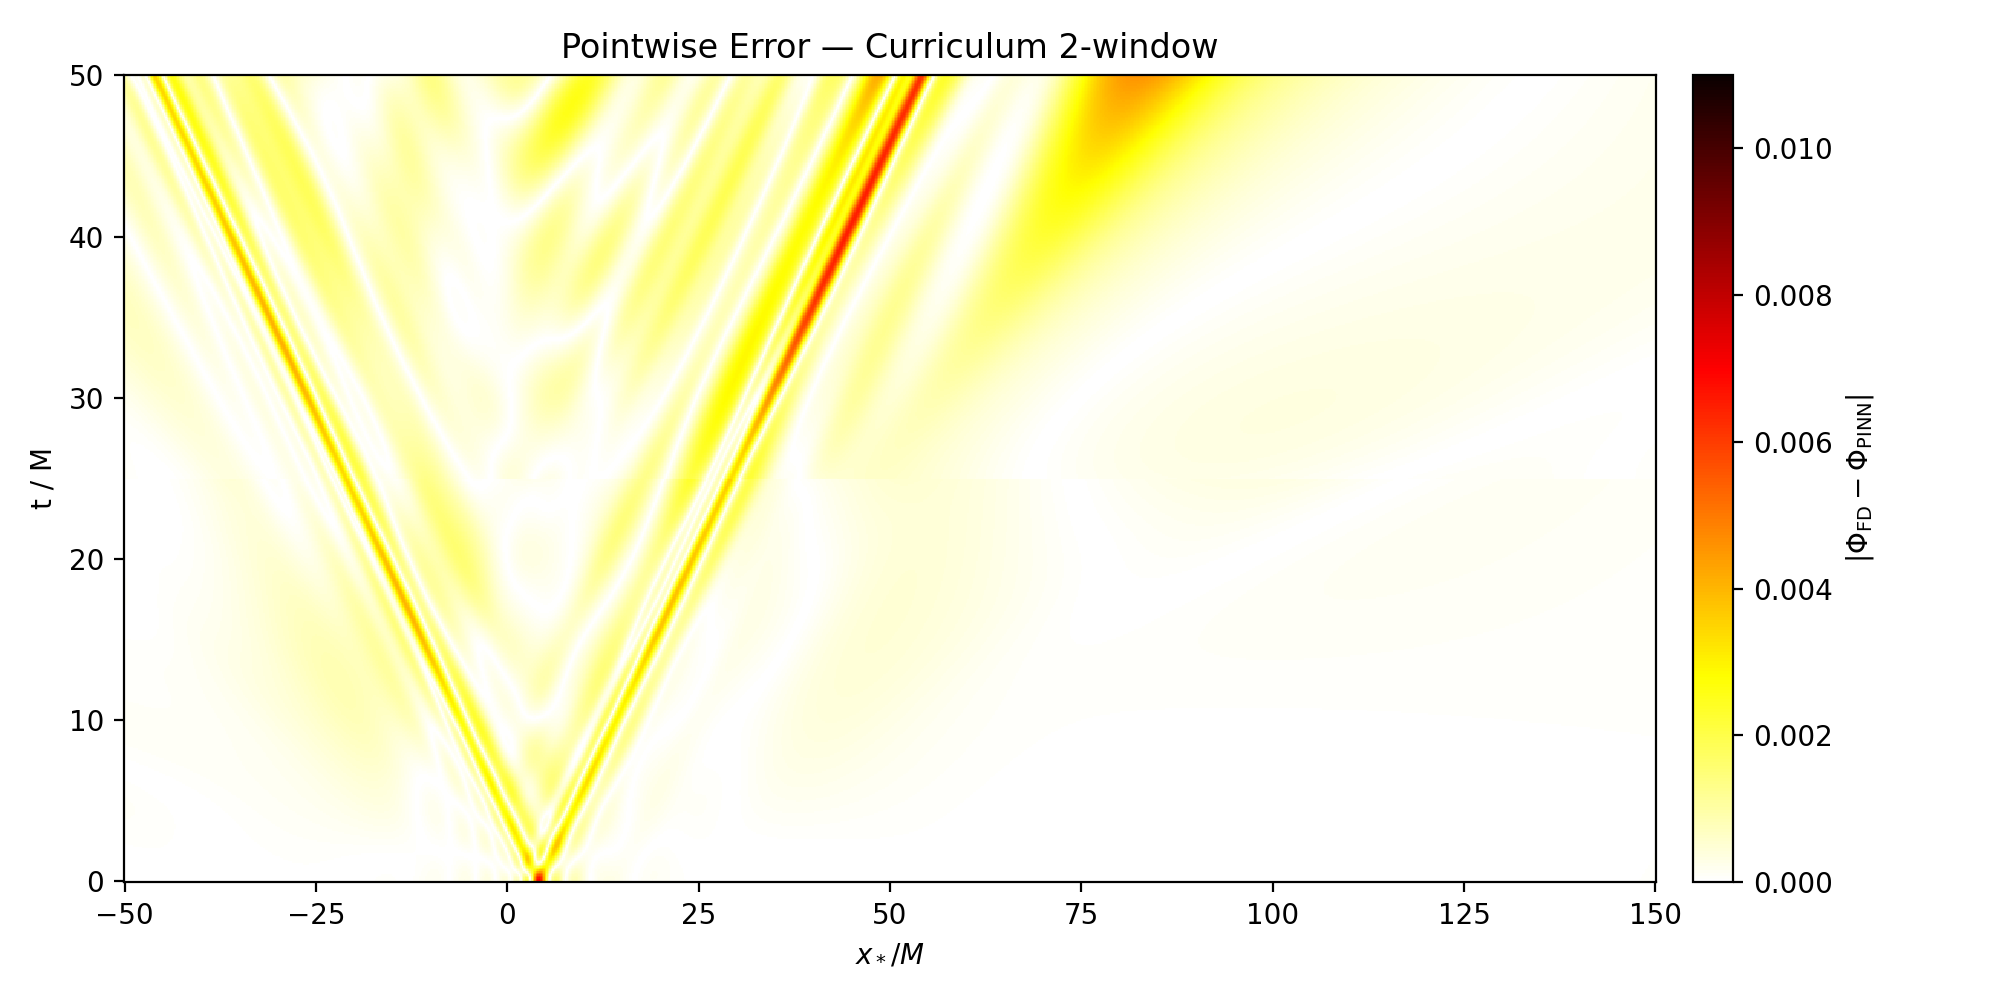
\includegraphics[width=\textwidth]{../outputs/pinn/zerilli_l2_curriculum/error_heatmap.png}
      \\{\tiny Curriculum 2-window}
    \end{column}
    \begin{column}{0.32\textwidth}
      \centering
      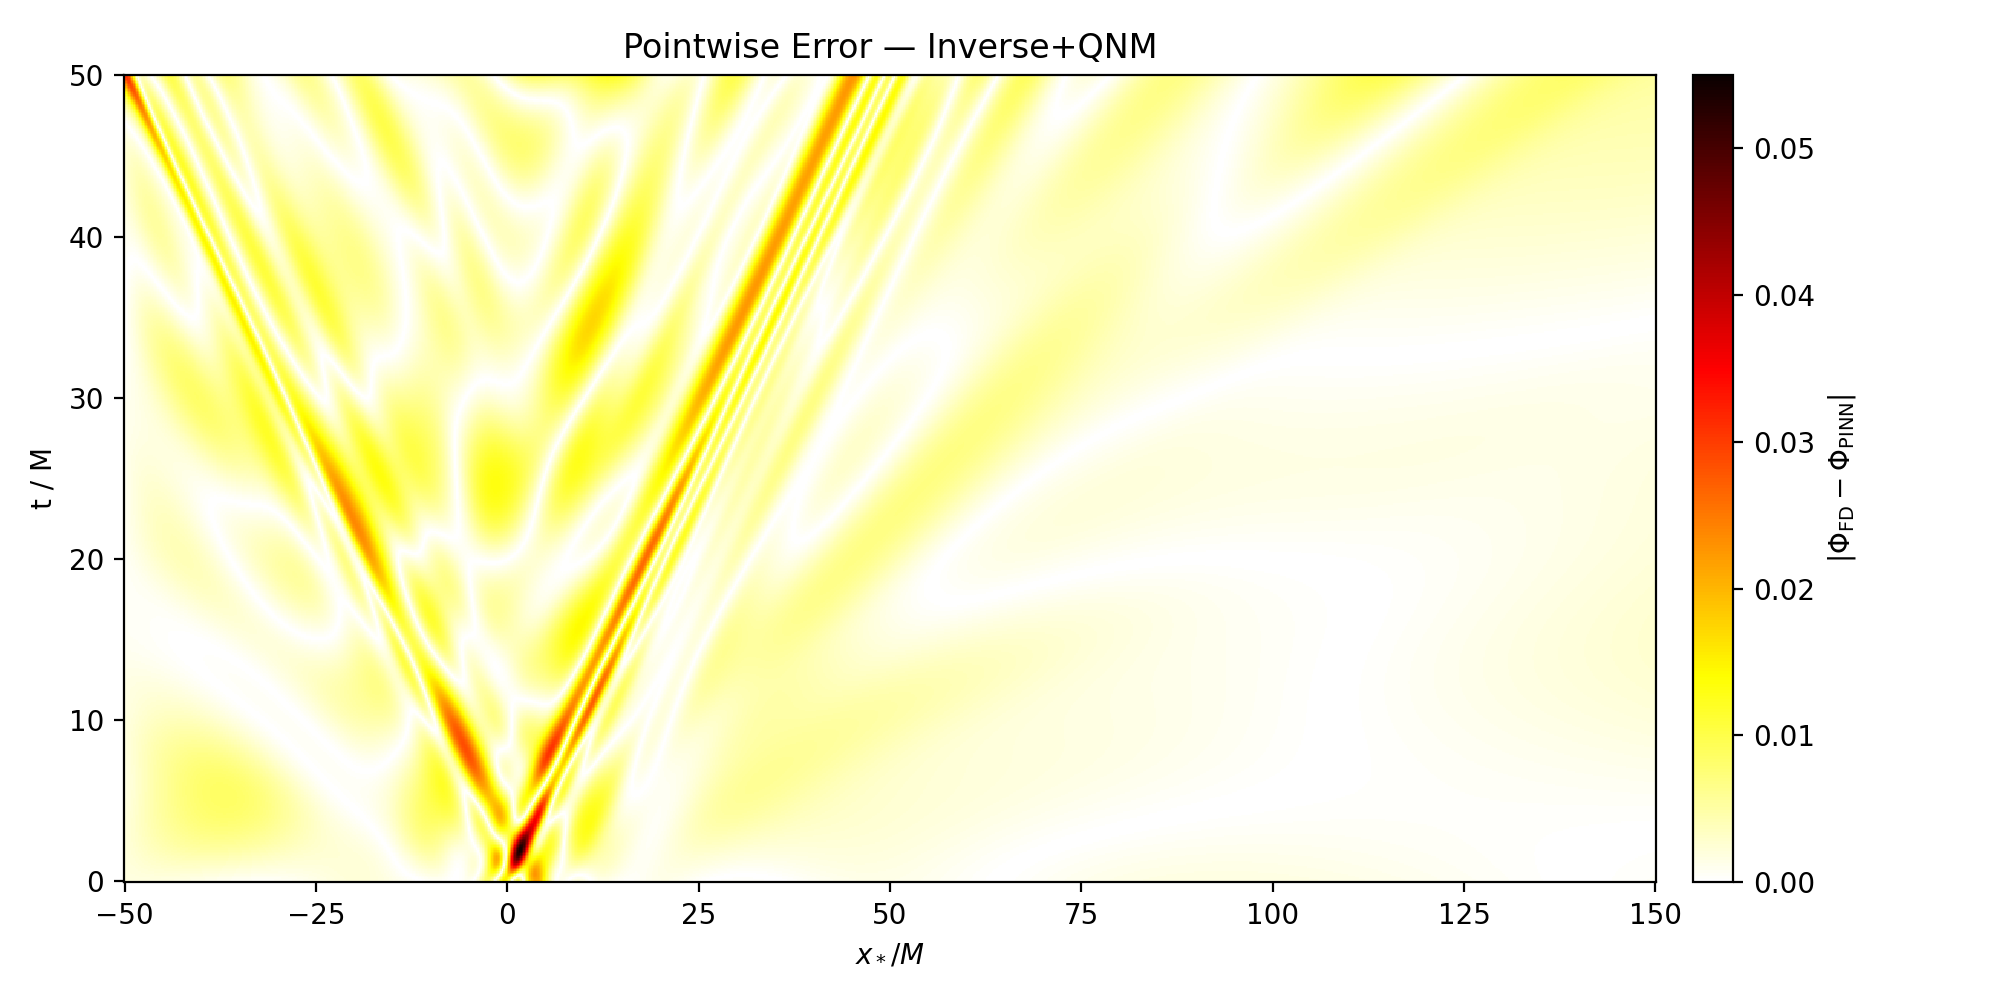
\includegraphics[width=\textwidth]{../outputs/pinn/zerilli_l2_inverse_qnm/error_heatmap.png}
      \\{\tiny Inverse PINN + Ringdown Template}
    \end{column}
  \end{columns}
\end{frame}

% --- Appendix: 3D Waveform ---
\begin{frame}{Appendix: 3D Waveform Visualisation}
  \begin{center}
    \includegraphics[width=0.85\textwidth,height=0.82\textheight,keepaspectratio]{../outputs/pinn/zerilli_l2_rad_k2/waveform_3d.png}
  \end{center}
\end{frame}

% --- Appendix: Loss Histories ---
\begin{frame}{Appendix: Loss History --- Baseline vs Greedy}
  \begin{columns}[T]
    \begin{column}{0.48\textwidth}
      \centering
      \includegraphics[width=\textwidth]{loss_reproduction.png}
      \\{\footnotesize Uniform baseline}
    \end{column}
    \begin{column}{0.48\textwidth}
      \centering
      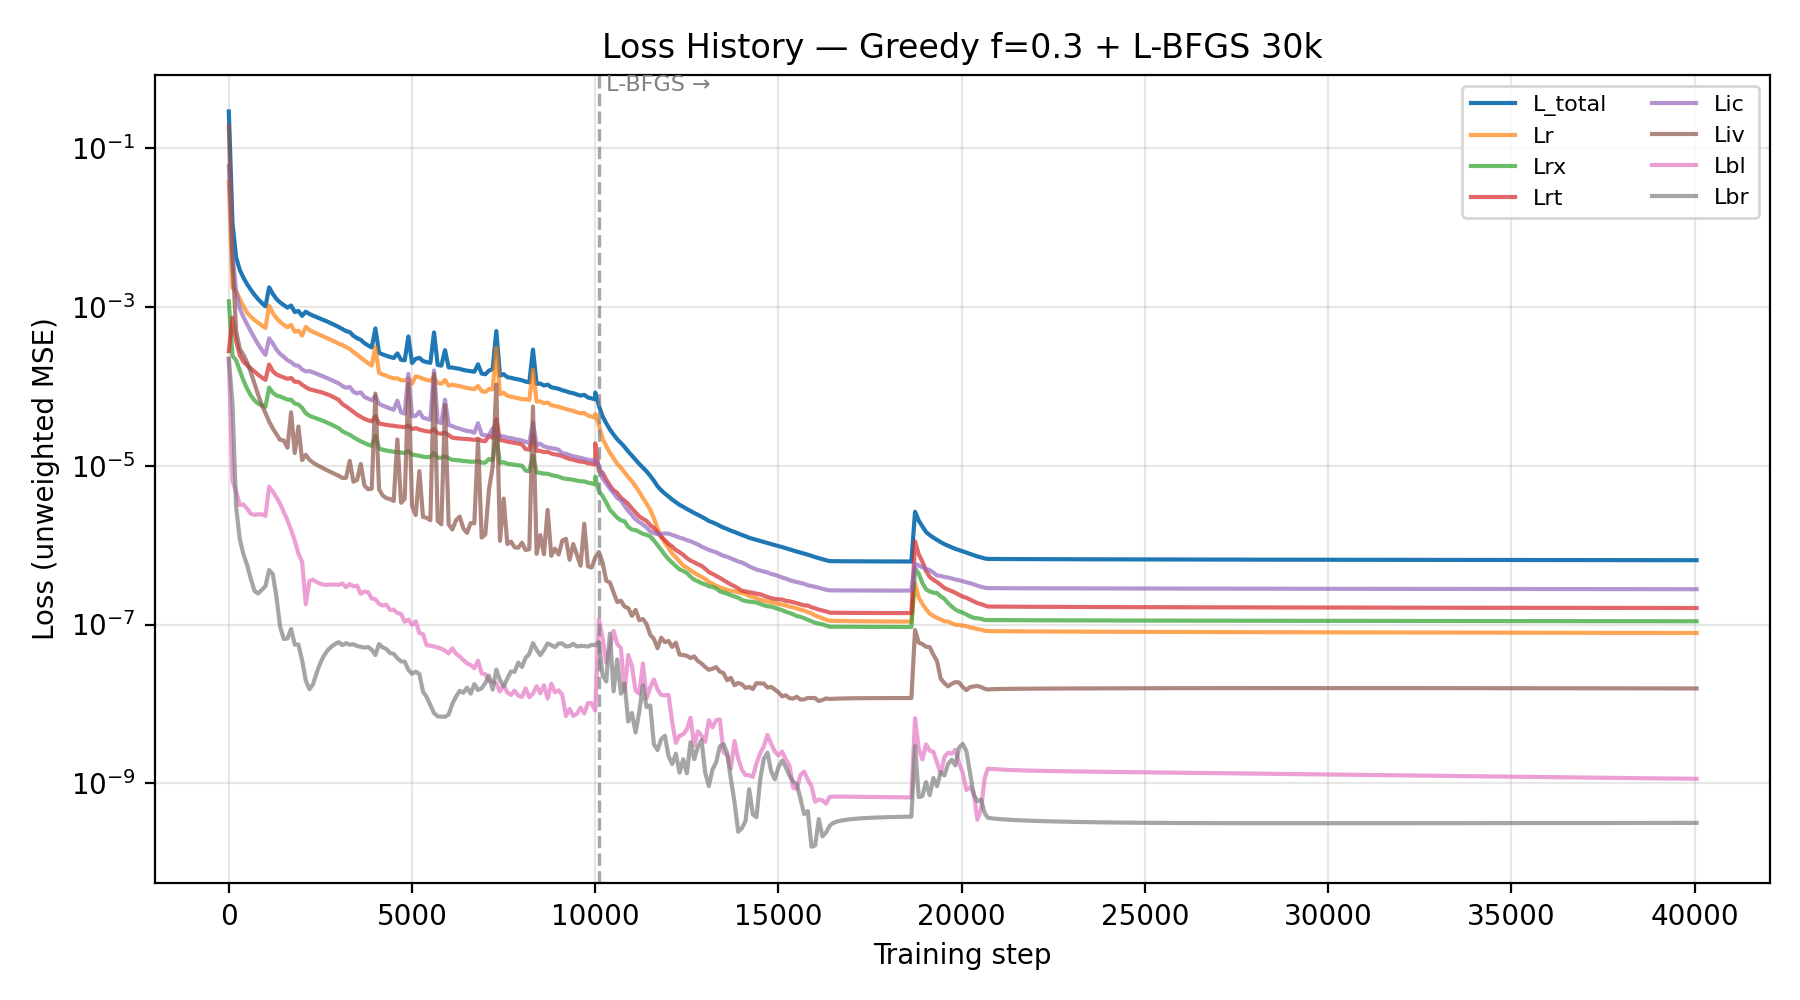
\includegraphics[width=\textwidth]{../outputs/pinn/zerilli_l2_greedy_f03_lbfgs30k/loss.png}
      \\{\footnotesize Greedy $f\!=\!0.3$ + L-BFGS 30k}
    \end{column}
  \end{columns}
\end{frame}

\end{document}
